%%%%%%%%%%%%%%%%% Willow Genotype by Environment Random Forest Analysis  %%%%%%%%%%%%%%%%%%%%%%%%%%%%%%%%%%%%%%%%
%%%%%%%%%%%%%%%%% Report for the analysis of Willow Experiments made in R studionand knitr %%%%%%%%%%%%%%%%%%%%%%
%%%%%%%%%%%%%%%%% Version 20150616

\documentclass{article}\usepackage[]{graphicx}\usepackage[]{color}
%% maxwidth is the original width if it is less than linewidth
%% otherwise use linewidth (to make sure the graphics do not exceed the margin)
\makeatletter
\def\maxwidth{ %
  \ifdim\Gin@nat@width>\linewidth
    \linewidth
  \else
    \Gin@nat@width
  \fi
}
\makeatother

\definecolor{fgcolor}{rgb}{0.345, 0.345, 0.345}
\newcommand{\hlnum}[1]{\textcolor[rgb]{0.686,0.059,0.569}{#1}}%
\newcommand{\hlstr}[1]{\textcolor[rgb]{0.192,0.494,0.8}{#1}}%
\newcommand{\hlcom}[1]{\textcolor[rgb]{0.678,0.584,0.686}{\textit{#1}}}%
\newcommand{\hlopt}[1]{\textcolor[rgb]{0,0,0}{#1}}%
\newcommand{\hlstd}[1]{\textcolor[rgb]{0.345,0.345,0.345}{#1}}%
\newcommand{\hlkwa}[1]{\textcolor[rgb]{0.161,0.373,0.58}{\textbf{#1}}}%
\newcommand{\hlkwb}[1]{\textcolor[rgb]{0.69,0.353,0.396}{#1}}%
\newcommand{\hlkwc}[1]{\textcolor[rgb]{0.333,0.667,0.333}{#1}}%
\newcommand{\hlkwd}[1]{\textcolor[rgb]{0.737,0.353,0.396}{\textbf{#1}}}%

\usepackage{framed}
\makeatletter
\newenvironment{kframe}{%
 \def\at@end@of@kframe{}%
 \ifinner\ifhmode%
  \def\at@end@of@kframe{\end{minipage}}%
  \begin{minipage}{\columnwidth}%
 \fi\fi%
 \def\FrameCommand##1{\hskip\@totalleftmargin \hskip-\fboxsep
 \colorbox{shadecolor}{##1}\hskip-\fboxsep
     % There is no \\@totalrightmargin, so:
     \hskip-\linewidth \hskip-\@totalleftmargin \hskip\columnwidth}%
 \MakeFramed {\advance\hsize-\width
   \@totalleftmargin\z@ \linewidth\hsize
   \@setminipage}}%
 {\par\unskip\endMakeFramed%
 \at@end@of@kframe}
\makeatother

\definecolor{shadecolor}{rgb}{.97, .97, .97}
\definecolor{messagecolor}{rgb}{0, 0, 0}
\definecolor{warningcolor}{rgb}{1, 0, 1}
\definecolor{errorcolor}{rgb}{1, 0, 0}
\newenvironment{knitrout}{}{} % an empty environment to be redefined in TeX

\usepackage{alltt}


%%%%%%%%%%%%%%%%% Load Lates Packages %%%%%%%%%%%%%%%%%%%%%%%%%%%%%%%%%%%%%%%%%%%%%%%%%%%%%%%%%%%%%%%%%%%%%%%%%%%

\usepackage[margin=1.0in]{geometry}

%%%%%%%%%%%%%%%%%% Set knitr Global Options, Install and load Packages used %%%%%%%%%%%%%%%%%%%%%%%%%%%%%%%%%%%%%%%%%%%%%



\IfFileExists{upquote.sty}{\usepackage{upquote}}{}
\begin{document}
\title{Willow Genotype by Environment\\ Random Forest Analysis}
\author{Felipe Montes - frm10@psu.edu}
\maketitle

%%%%%%%%%%%%%%%%% Insert and introduction Section Explaining the Analysis %%%%%%%%%%%%%%%%%%%%%%%%%%%%%%%%%%%%%%%

\section*{Introduction}

The following random forest analysis was based on the Willow Experimental database that Eric passed to me on 03/18/2015. I did not know the database in detail, therefore the firsts steps in the analysis are on understanding the data base, where gaps are, identifying mistakes and typos and cleaning the database for further analysis.



\section*{Describing the Database}

The database had when read into R 60 different variables and 1800 observations.

Establish Year,  Harvest Year,  Trial ID,	Site (SAS),	Rep,	Clone ID,	Epithet,	Family,	New Diversity Group,	Clone (SAS),	Ploidy level,	Survival (\%),	Surviv prop,	Wet Yield (Mg/ha),	Biomass \% Moisture,	Biomass Moisture prop,	Biomass \% dry matter,	Biomass dry matter prop,	Dry Yield (Mg/ha),	Annual Yield (Mg/ha/yr),	Dry tons/ac,	Dry tons/ac/yr,	\% Hemicellulose,	\% Cellulose,	\% Lignin,	\% Ash,	Density (g/cm3),	Od volume (m3),	Hemicellulose yield, Cellulose yield,	Lignin yield,	Ash yield,	\% Organic Matter,	Soil pH,	[H+],	Soil P (mg/kg),	Soil K (mg/kg),	Soil Ca (mg/kg),	Soil Mg (mg/kg),	Soil Fe (mg/kg),	Soil Mn (mg/kg),	Soil Zn (mg/kg),	Soil Al (mg/kg),	Mean ann prcp (mm),	Mean ann GDD (base 10oC),	Prcp: April-Oct (mm),	Tmax: April-Oct(oC),	Annual Tmin (oC),	Annual solar radiation (MJ m-1 day-1),	Solar radiation: Apr-Oct (MJ m-1 d-1),	Elevation (ft),	Elevation (m),	Depth to water table-low(cm),	Depth to Water Table-high(cm),	Available water capacity (cm/cm),	Land capability class,	LC subclass,	Height (m),	Area per plot (cm2),	Comments.\\

Many of the variables are the same variable coded with different name or different units i.e. Dry Yield (Mg/ha),  Annual Yield (Mg/ha/yr),	Dry tons/ac,	Dry tons/ac/yr; many of those variables are correlated in some way or another i.e. Dry Yield (Mg/ha), Wet Yield (Mg/ha) or Site (SAS), Trial ID. or Clone ID,  Epithet,	Family,	New Diversity Group,	Clone (SAS),	Ploidy level. Variable Site (SAS) is related to the Trial ID, Rep, Elevation (m),  Depth to water table-low(cm),	Depth to Water Table-high(cm),	Available water capacity (cm/cm),	Land capability class,	LC subclass,    the soils variables (\% Organic Matter,  Soil pH,	[H+],	Soil P (mg/kg),	Soil K (mg/kg),	Soil Ca (mg/kg),	Soil Mg (mg/kg),	Soil Fe (mg/kg),	Soil Mn (mg/kg),	Soil Zn (mg/kg),	Soil Al (mg/kg)) as well as weather variables (Mean ann prcp (mm),  Mean ann GDD (base 10oC),  Prcp: April-Oct (mm),	Tmax: April-Oct(oC),	Annual Tmin (oC),	Annual solar radiation (MJ m-1 day-1),	Solar radiation: Apr-Oct (MJ m-1 d-1)). While soils variables do not vary within location, weather variables  do vary within location each year. Therefore, even though location determines the weather, each year has different weather on each location. At the same time, Year is also related to weather, as during one year the weather conditions will have similar pattern across locations, but also will vary within one location.\\

Additionally, many observations have significant information gaps; typos and missing data. \\

Random Forest is very flexible and accommodating tool for analysis, it can impute missing data based on the whole database, but  it makes no sense to apply it blindly to the database as is.\\


Therefore variables year and location were separated into two different variables
More about correlations will be discussed later.

\subsection*{Variable Groups}

In order to facilitate the analysis variables were grouped as follows:\\

\begin{itemize}
  \item
  Descriptor variables: "Establish.Year","Harvest.Year","Trial.ID","Site..SAS.","Elevation..m.", "Location","Rep","Area.per.plot..cm2."
  
  \item
  Predictor variables(continuous): "X..Organic.Matter", "Soil.pH", "X.H..", "Soil.P..mg.kg.", "Soil.K..mg.kg.", "Soil.Ca..mg.kg.","Soil.Mg..mg.kg.", "Soil.Fe..mg.kg.", "Soil.Mn..mg.kg.", "Soil.Zn..mg.kg.","Soil.Al..mg.kg.", "Mean.ann.prcp..mm.", "Mean.ann.GDD..base.10oC.", "Prcp..April.Oct..mm.", "Tmax..April.Oct.oC.", "Annual.Tmin..oC.", "Annual.solar.radiation..MJ.m.1.day.1.", "Solar.radiation..Apr.Oct..MJ.m.1.d.1.","Depth.to.water.table.low.cm.", "Depth.to.Water.Table.high.cm.", "Available.water.capacity..cm.cm." , "Height..m." and "Od.volume..m3."
  
  \item
  Predictor variables(factors) :"Clone.ID","Epithet","Family","New.Diversity.Group","Clone..SAS.","Ploidy.level","Land.capability.class","LC.subclass".
  
  \item
  Response.variables: "Survival....","Surviv.prop","Wet.Yield..Mg.ha.","Biomass...Moisture","Biomass.Moisture.prop","Biomass...dry.matter","Biomass.dry.matter.prop","Dry.Yield..Mg.ha.","Annual.Yield..Mg.ha.yr.","Dry.tons.ac","Dry.tons.ac.yr","X..Hemicellulose","X..Cellulose","X..Lignin", "X..Ash", "Density..g.cm3.", "Hemicellulose.yield", "Cellulose.yield", "Lignin.yield", "Ash.yield".
  
\end{itemize}

Descriptor Variables with exception of Elevation are treated as factors, as are the Predictor variables(factors). Both response variables and predictor variables(continuous) are treated as numeric continuous variables

\subsection*{Missing values, Typos and other errors}

The database can be characterized by identifying variables that have many missing observations, or typos. To explore which variables have many missing values histograms indicating the number of missing values give a first glance

  
\begin{knitrout}
\definecolor{shadecolor}{rgb}{0.969, 0.969, 0.969}\color{fgcolor}

{\centering 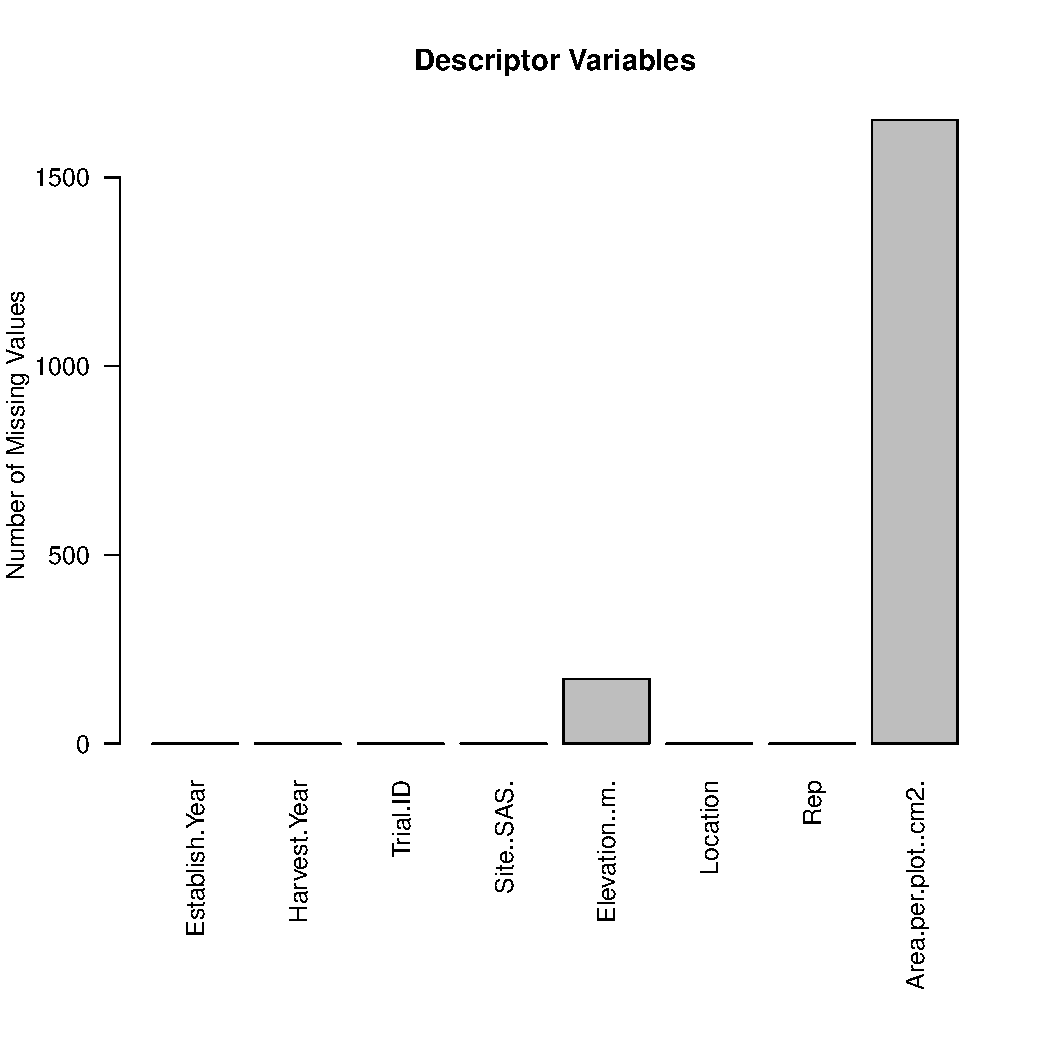
\includegraphics[width=\maxwidth]{figure/MissingValuesPredictorGroup-1} 

}




{\centering 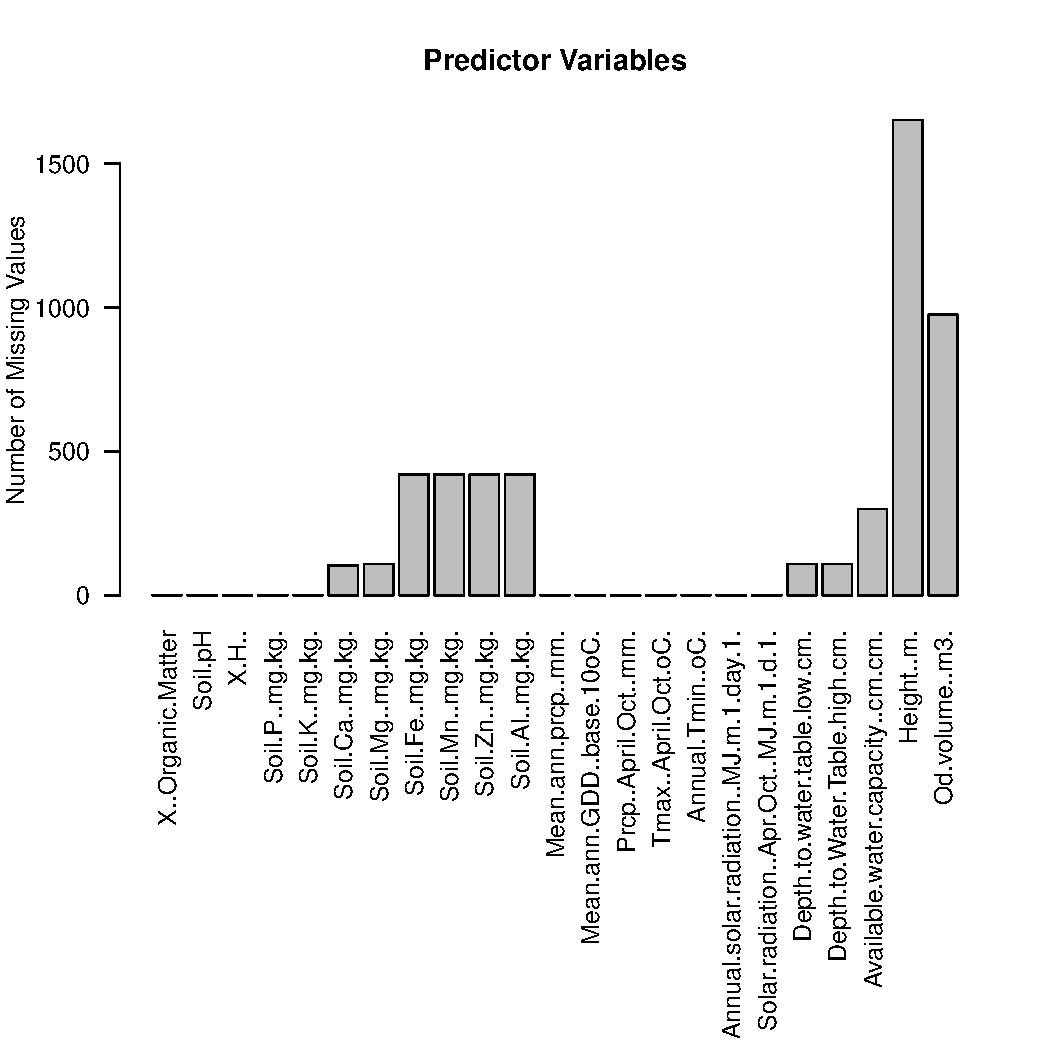
\includegraphics[width=\maxwidth]{figure/MissingValuesPredictorGroup-2} 

}




{\centering 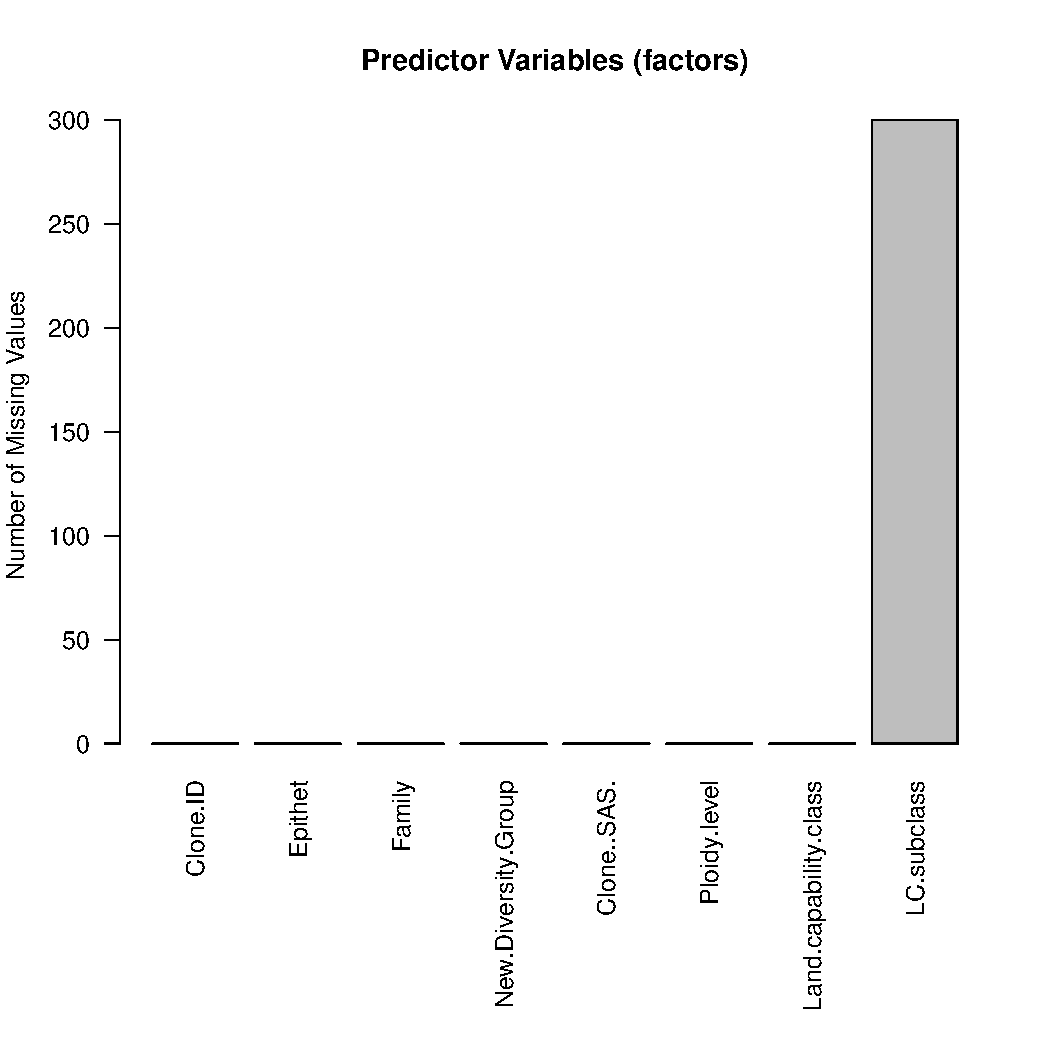
\includegraphics[width=\maxwidth]{figure/MissingValuesPredictorGroup-3} 

}




{\centering 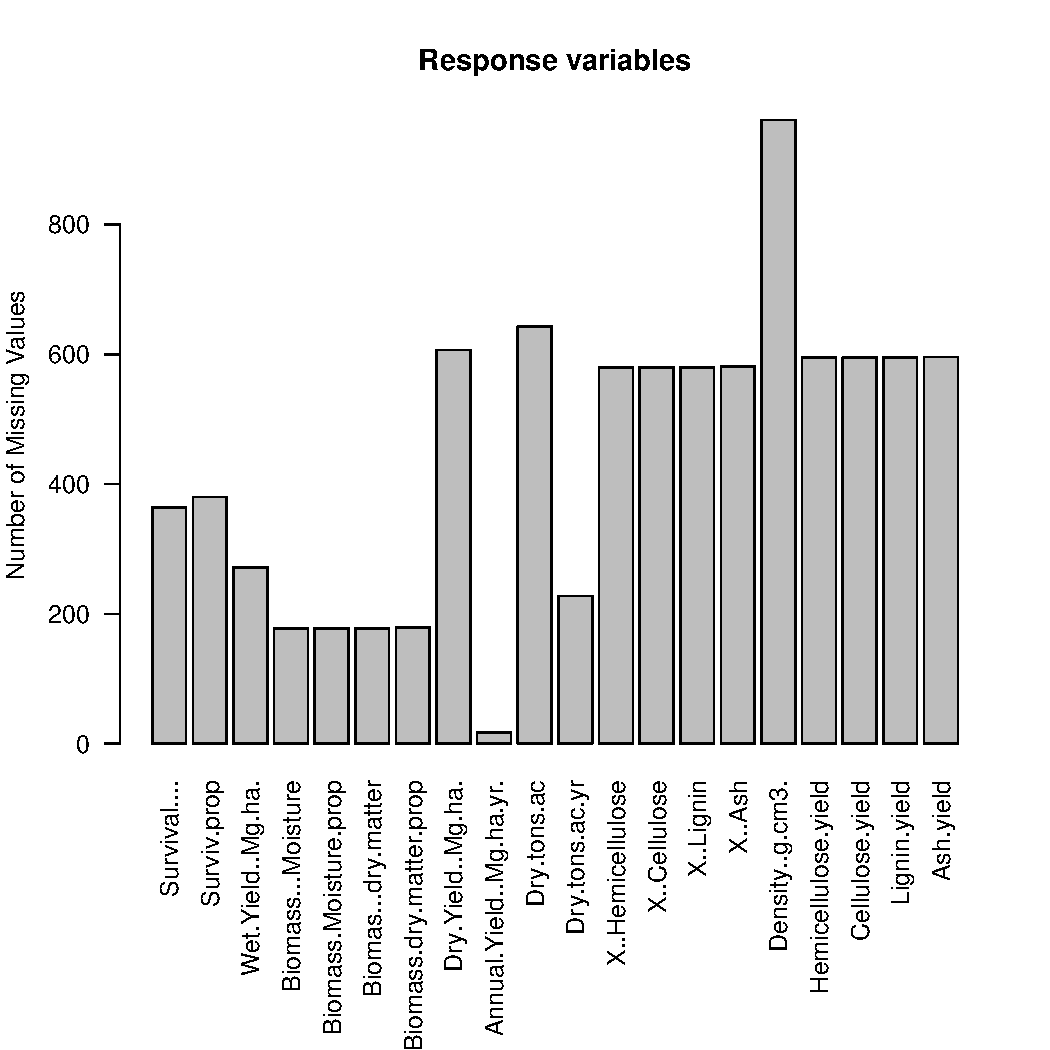
\includegraphics[width=\maxwidth]{figure/MissingValuesPredictorGroup-4} 

}



\end{knitrout}

There are several variables with large data gaps, how should we handle them? Should we exclude variables that have large data gaps? Should we impute them?\\

A strategy to look for typos and errors is to plot histograms of the variables to identify factor levels or continuous variable partitions that have small number of counts. In this way if a typo occurs in only one factor variable, that typo would create a new level of the factor with only one count on that level, the one that the typo generated. If we do this for the important group variables we get the following.\newpage


\subsubsection*{Descriptor Variables} 


\begin{knitrout}
\definecolor{shadecolor}{rgb}{0.969, 0.969, 0.969}\color{fgcolor}

{\centering 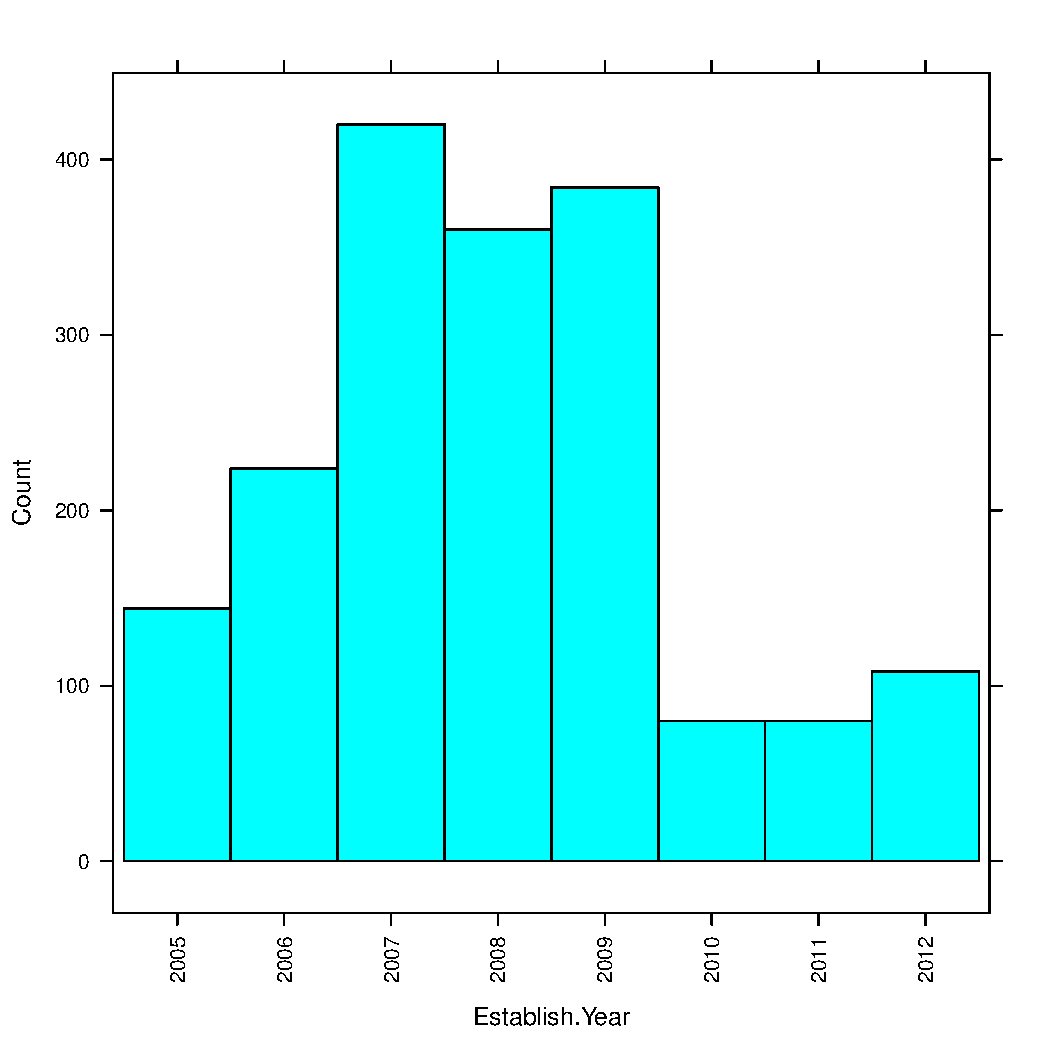
\includegraphics[width=\maxwidth]{figure/HistogramsDescriptorVariables-1} 

}




{\centering 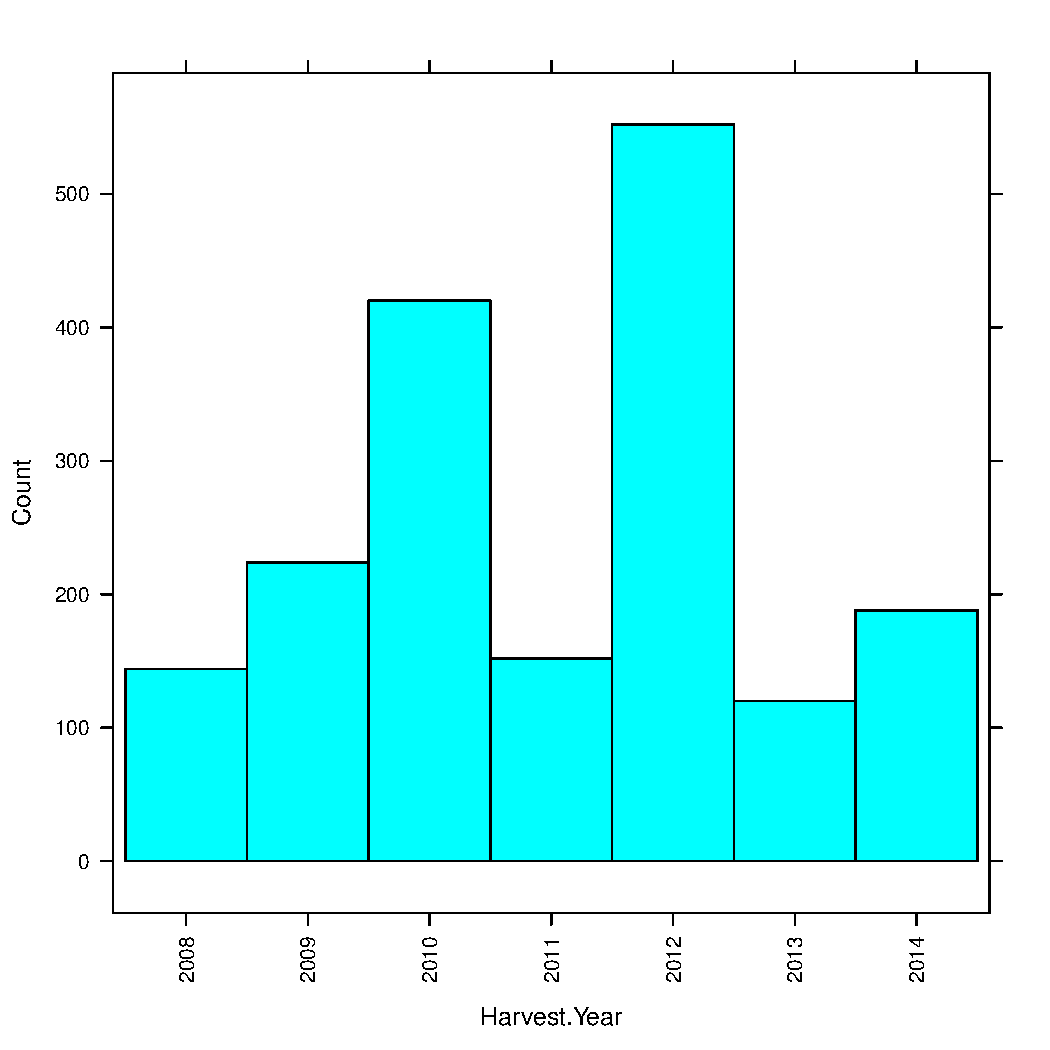
\includegraphics[width=\maxwidth]{figure/HistogramsDescriptorVariables-2} 

}




{\centering 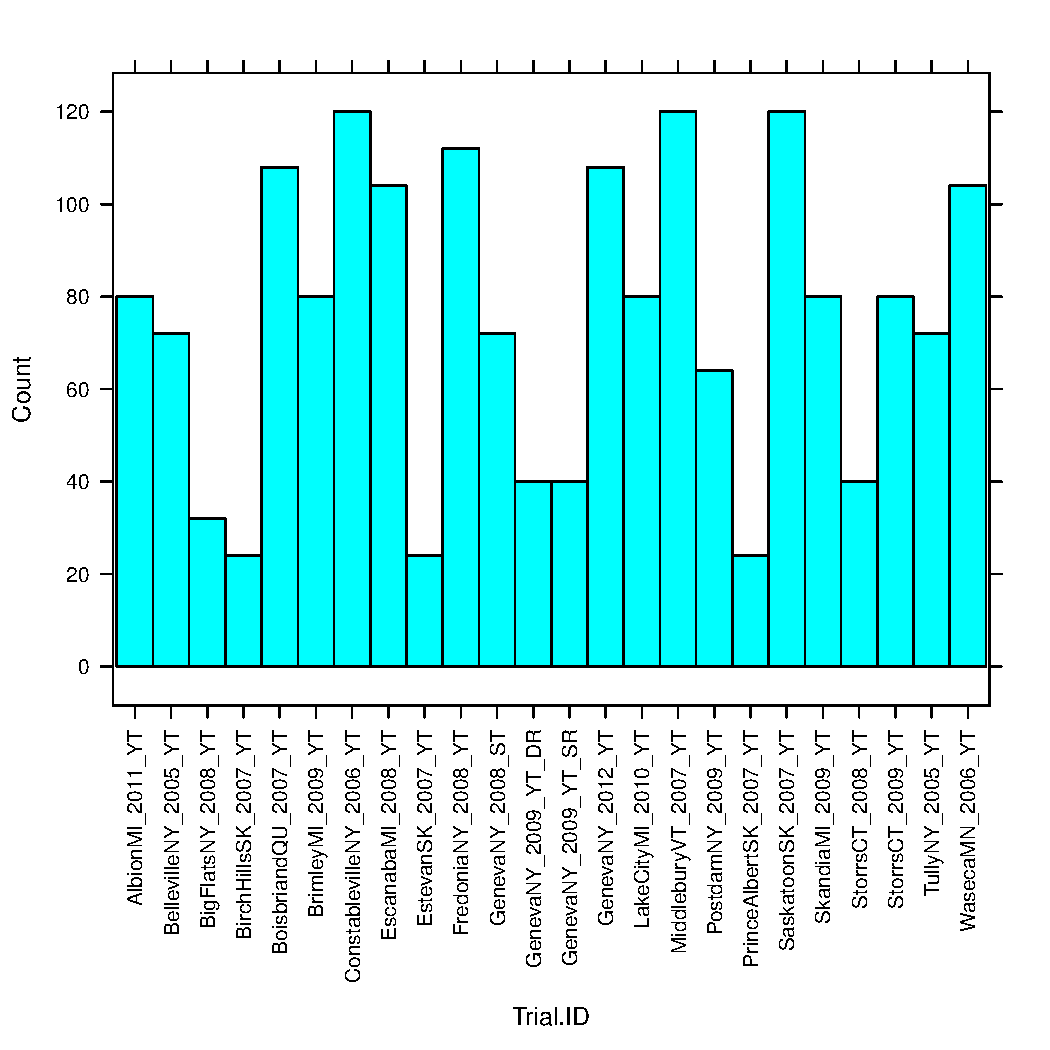
\includegraphics[width=\maxwidth]{figure/HistogramsDescriptorVariables-3} 

}




{\centering 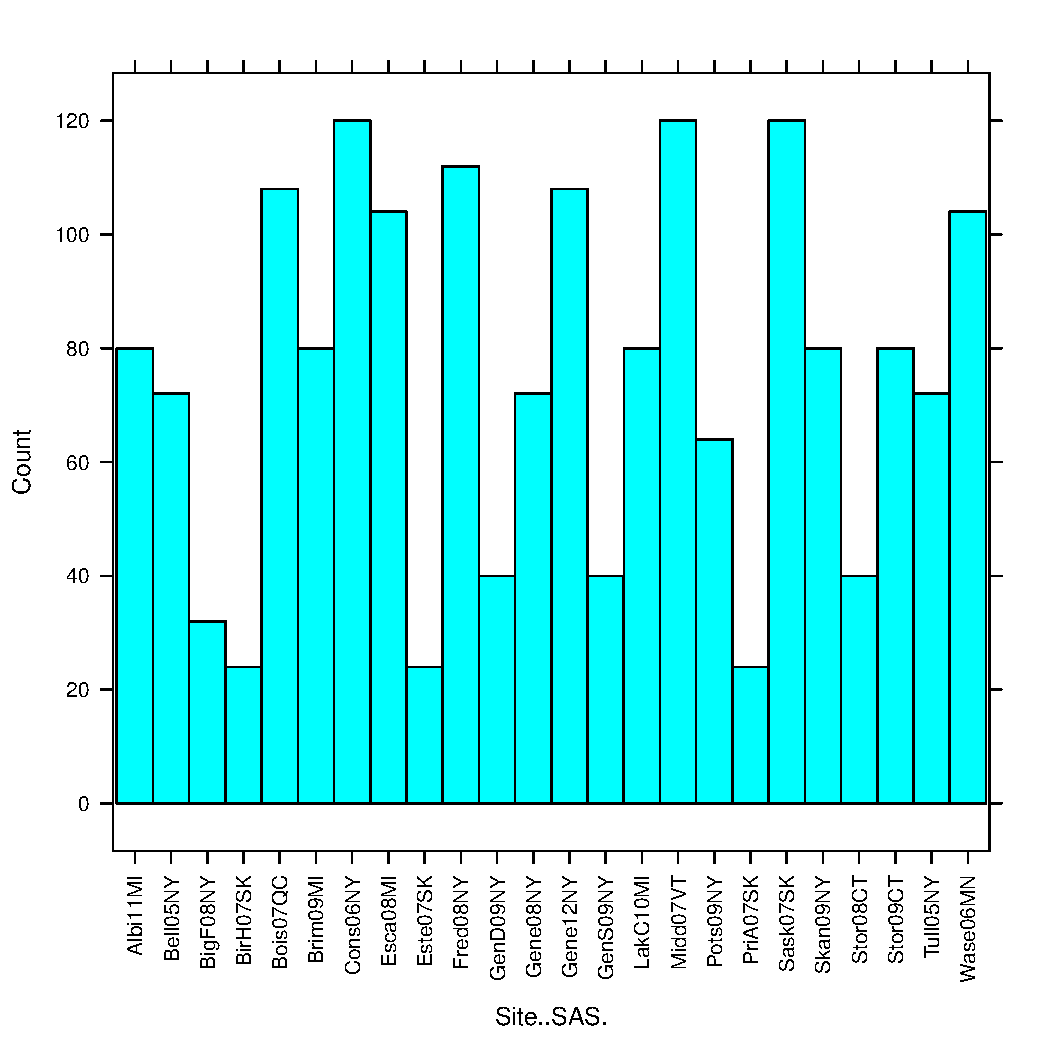
\includegraphics[width=\maxwidth]{figure/HistogramsDescriptorVariables-4} 

}




{\centering 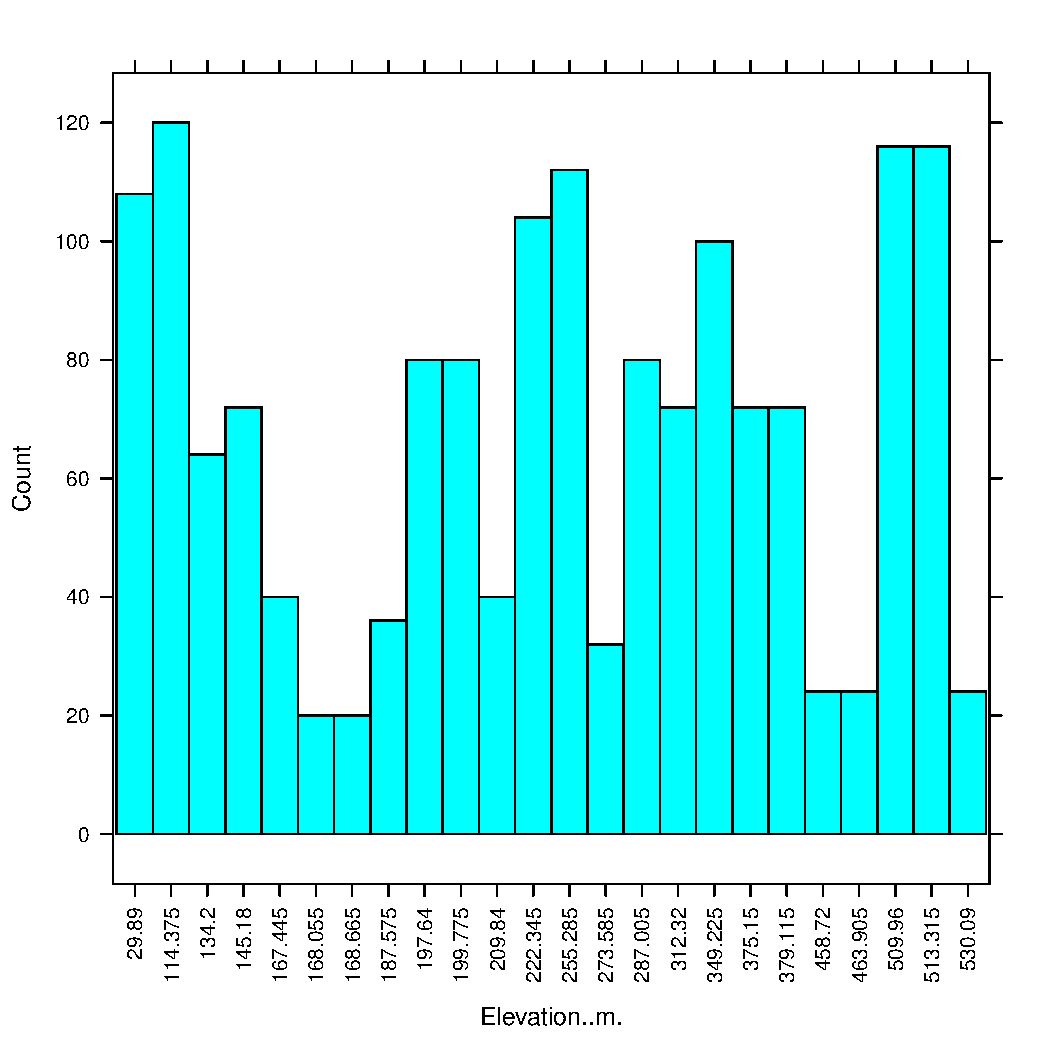
\includegraphics[width=\maxwidth]{figure/HistogramsDescriptorVariables-5} 

}




{\centering 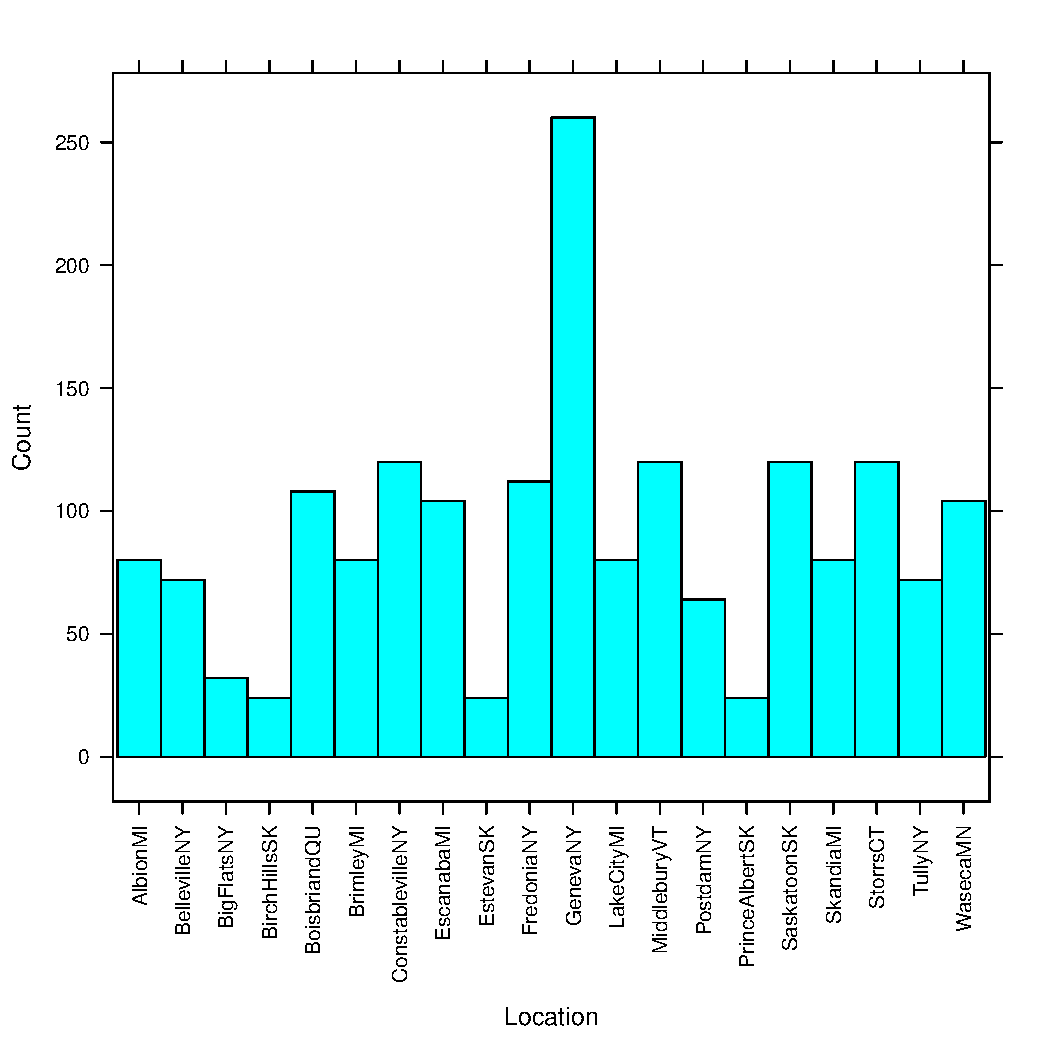
\includegraphics[width=\maxwidth]{figure/HistogramsDescriptorVariables-6} 

}




{\centering 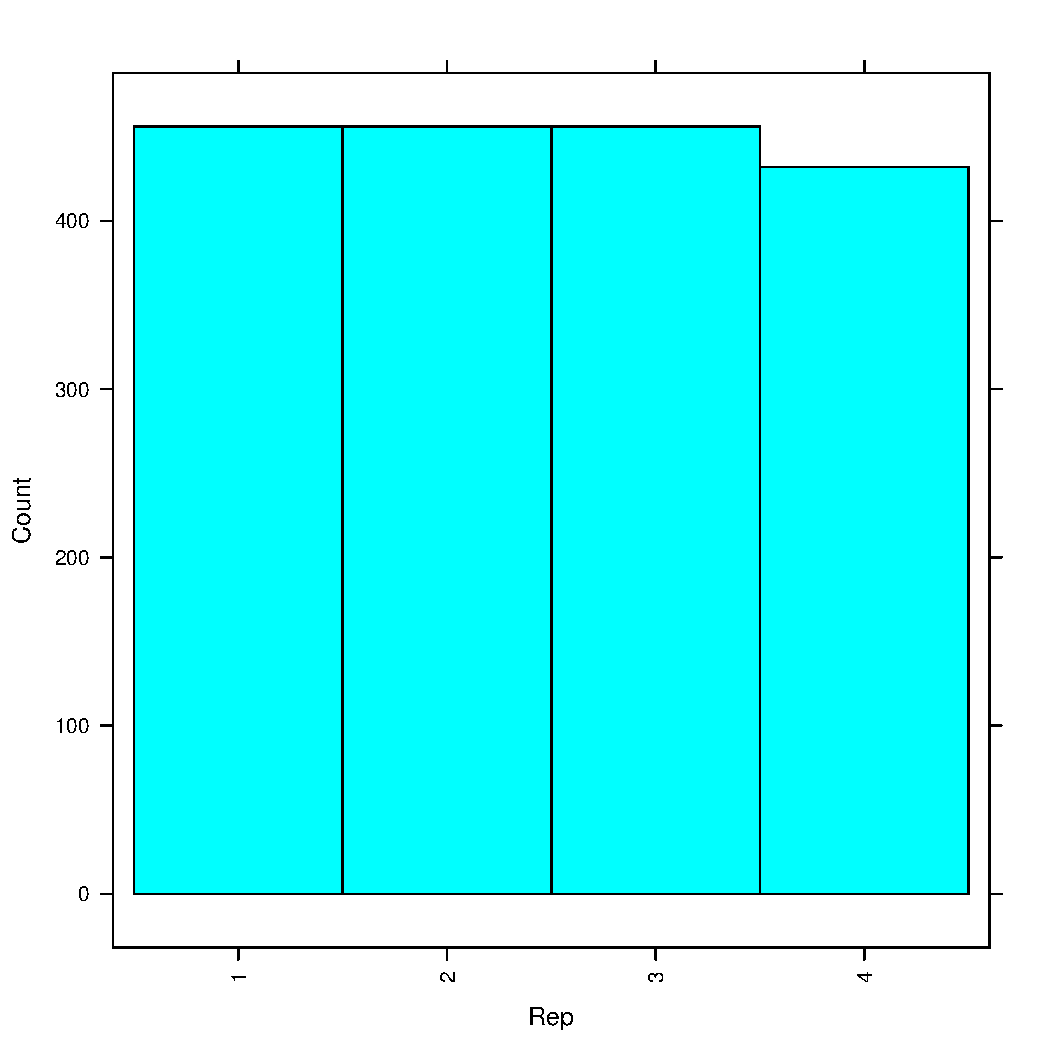
\includegraphics[width=\maxwidth]{figure/HistogramsDescriptorVariables-7} 

}



\end{knitrout}

From the histograms of the distribution of values in the descriptor group there is much that can be interpreted form the database. Few important things are:


\begin{itemize}

  \item
  There have been fewer experiments planted since 2010 and therefore the database is unbalanced with respect to establishment year; from 2005 to 2009, and 2010 and after
  
  \item
  Except for years 2010 and 2012, harvest years appear to be more balanced; what is the reason for it? 
  
  \item
  There are important differences in trial data entries, which will bias the result toward trials with more data entries as these have more data to contribute to the analysis; this is also the case for sites and its related variables 
  
  
\end{itemize}

\newpage

\subsubsection*{Predictor Variables} 


\begin{knitrout}
\definecolor{shadecolor}{rgb}{0.969, 0.969, 0.969}\color{fgcolor}

{\centering 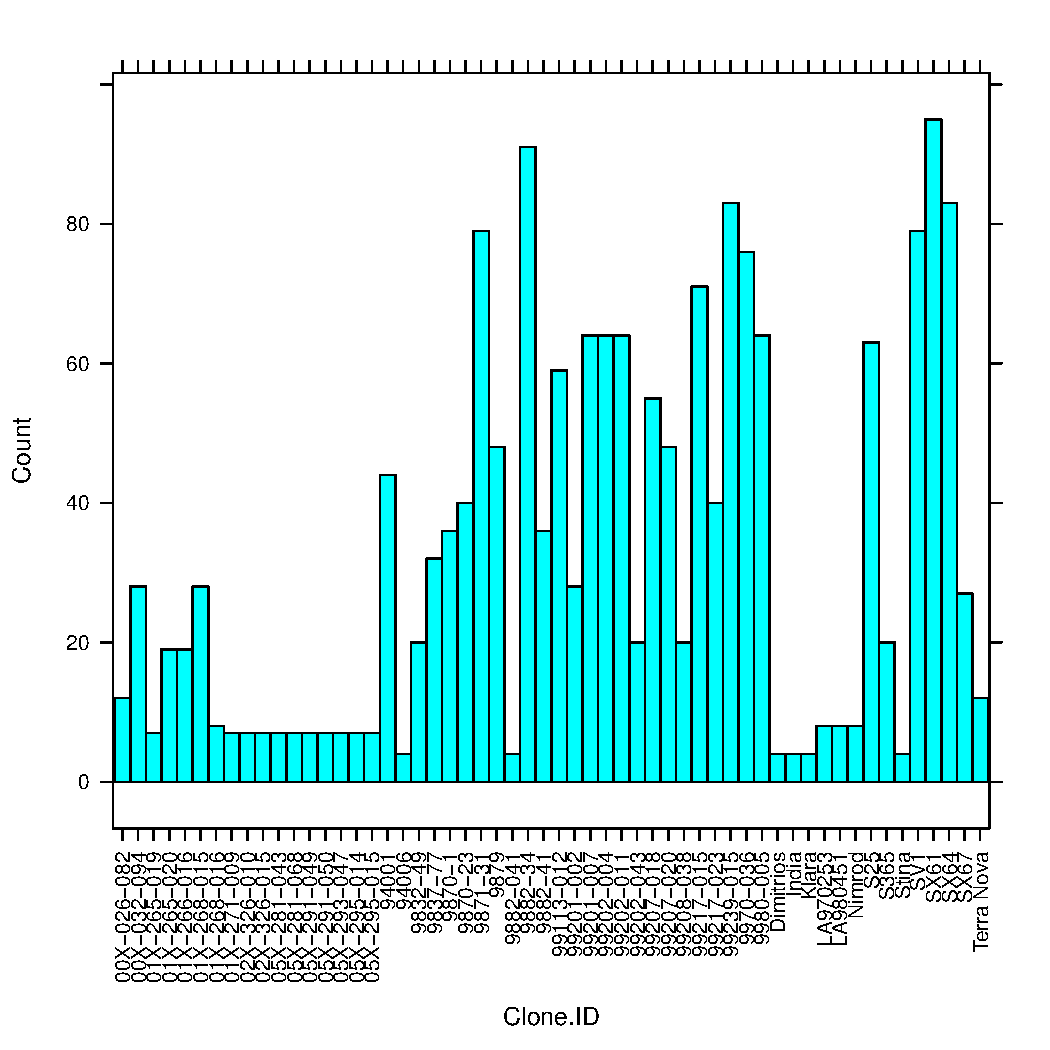
\includegraphics[width=\maxwidth]{figure/HistogramsPredictorVariables-1} 

}




{\centering 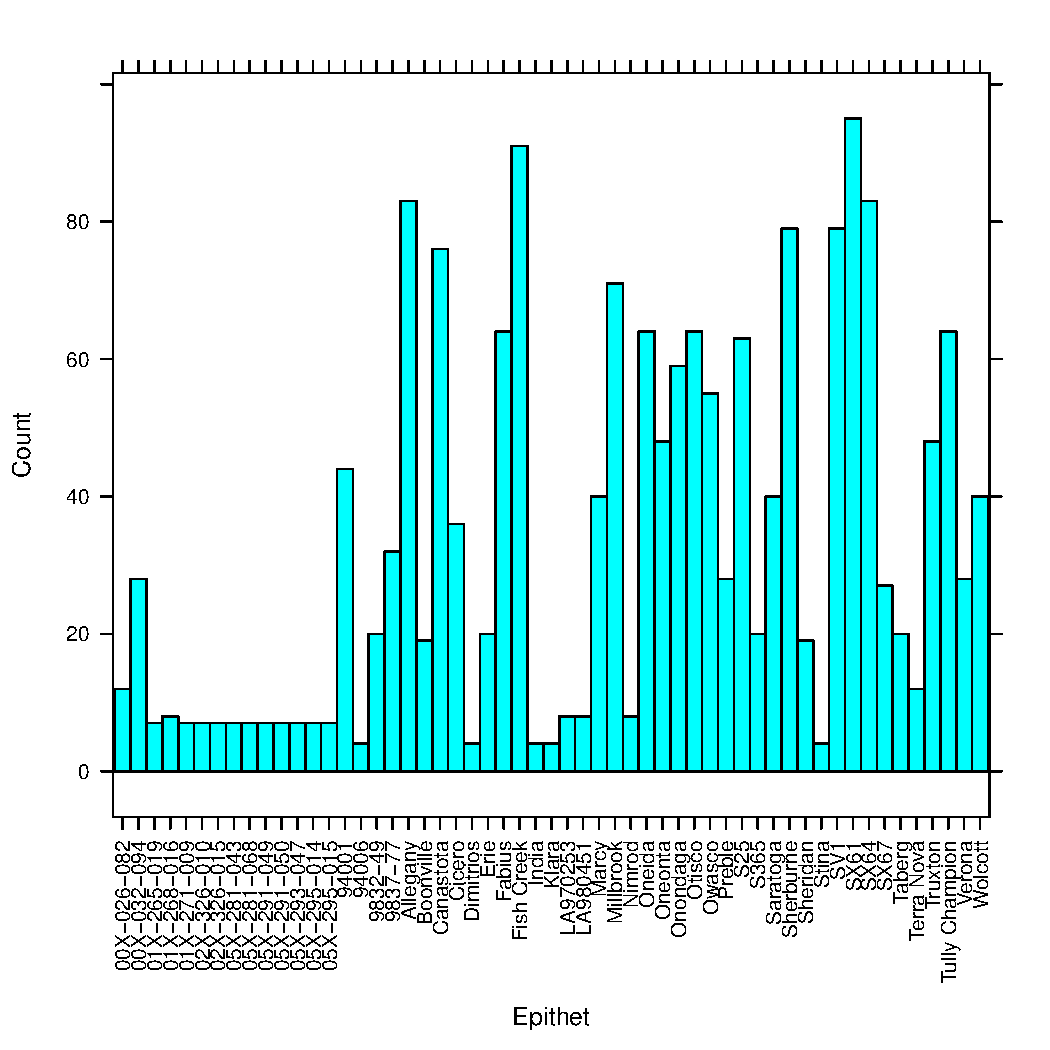
\includegraphics[width=\maxwidth]{figure/HistogramsPredictorVariables-2} 

}




{\centering 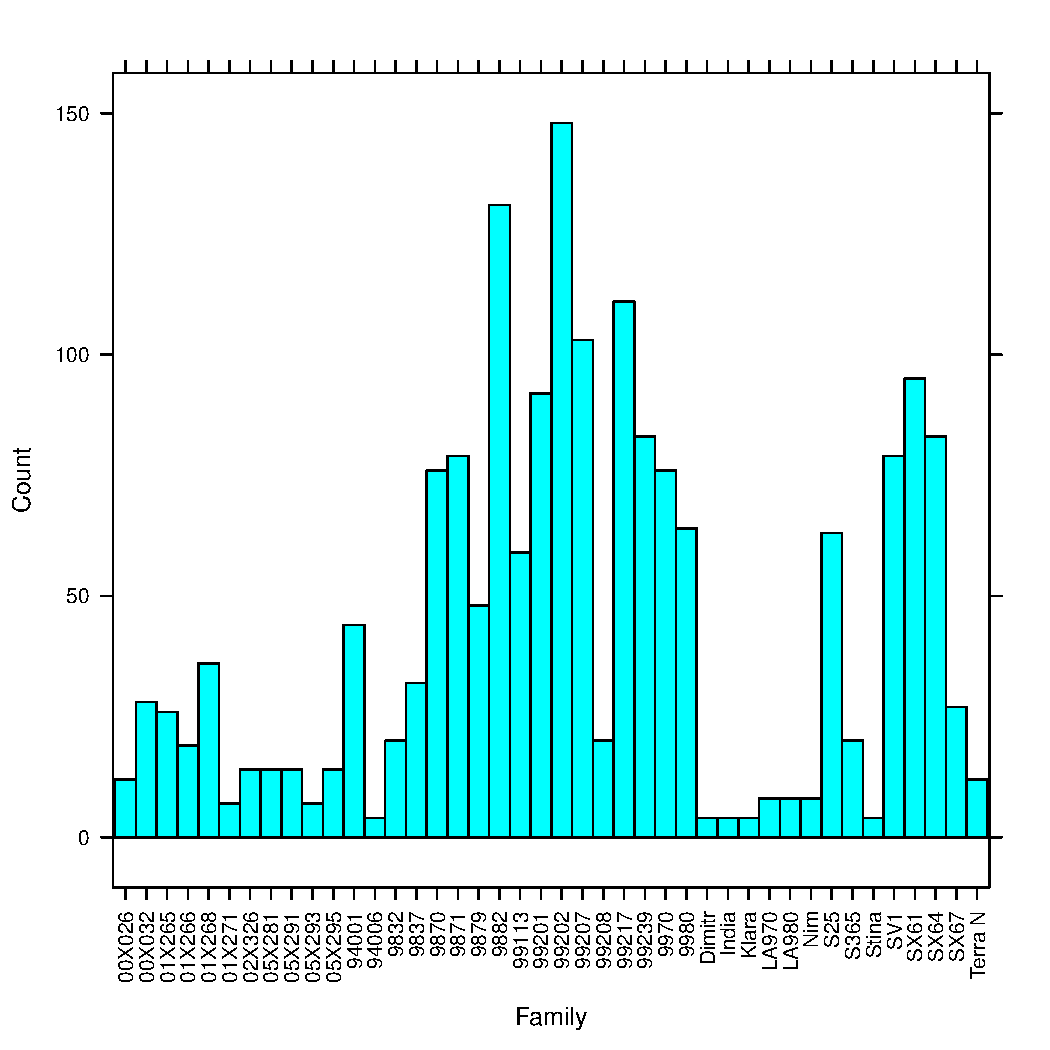
\includegraphics[width=\maxwidth]{figure/HistogramsPredictorVariables-3} 

}




{\centering 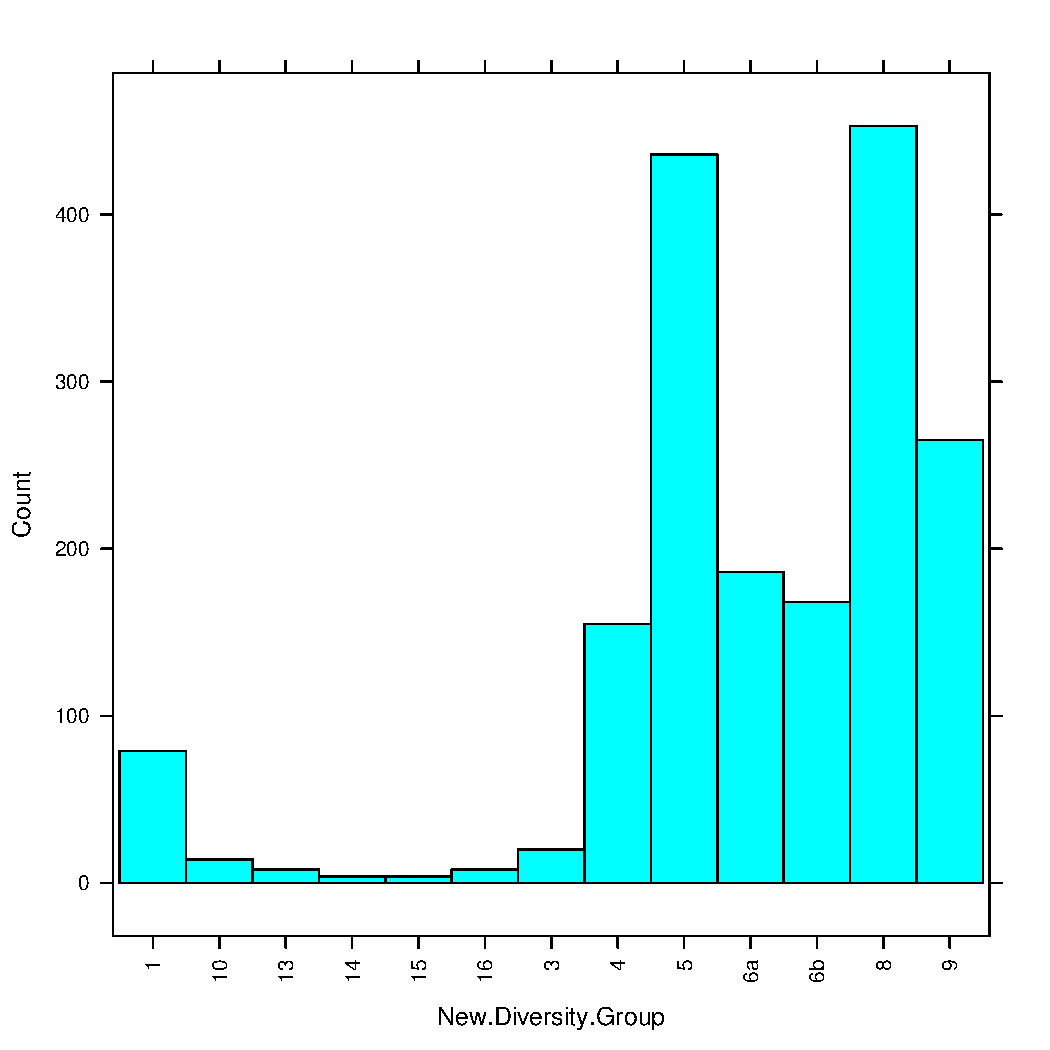
\includegraphics[width=\maxwidth]{figure/HistogramsPredictorVariables-4} 

}




{\centering 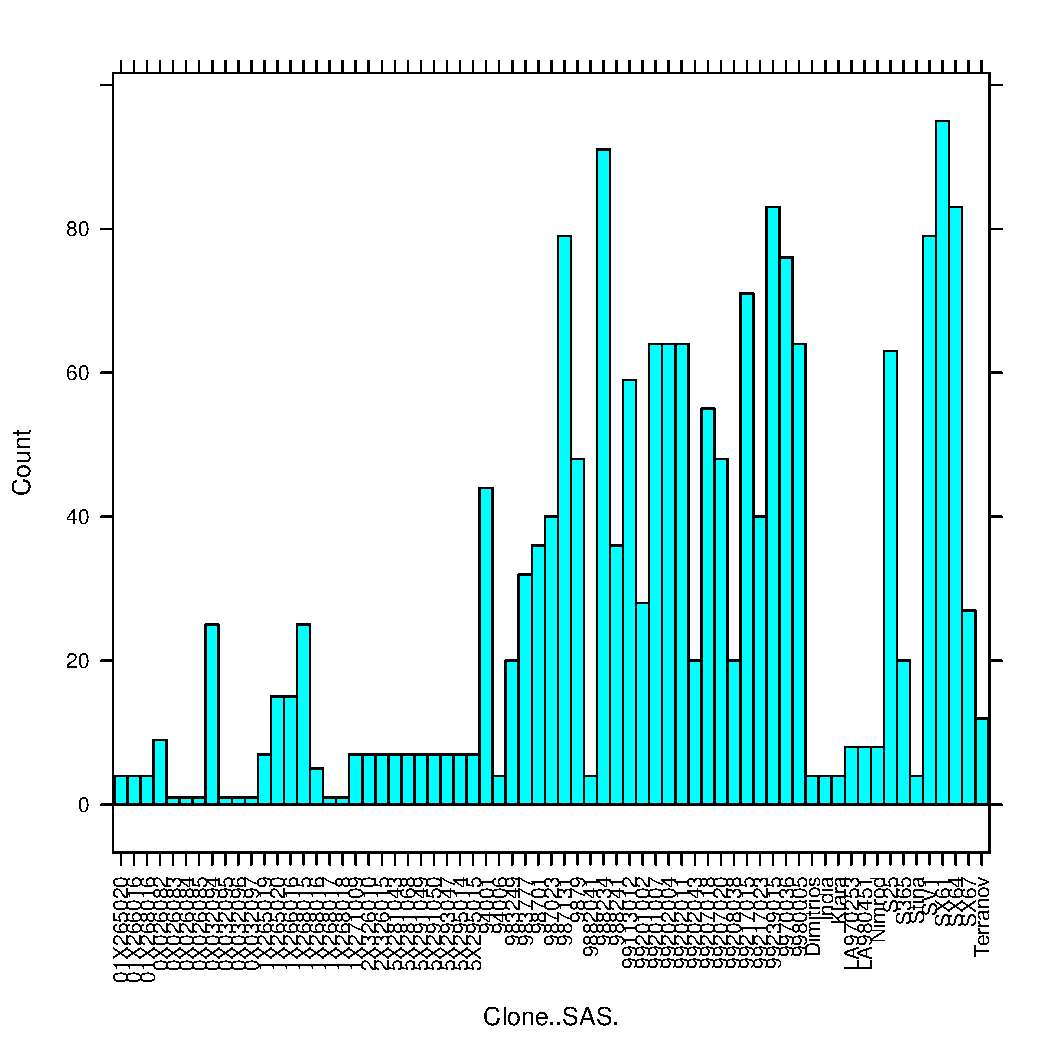
\includegraphics[width=\maxwidth]{figure/HistogramsPredictorVariables-5} 

}




{\centering 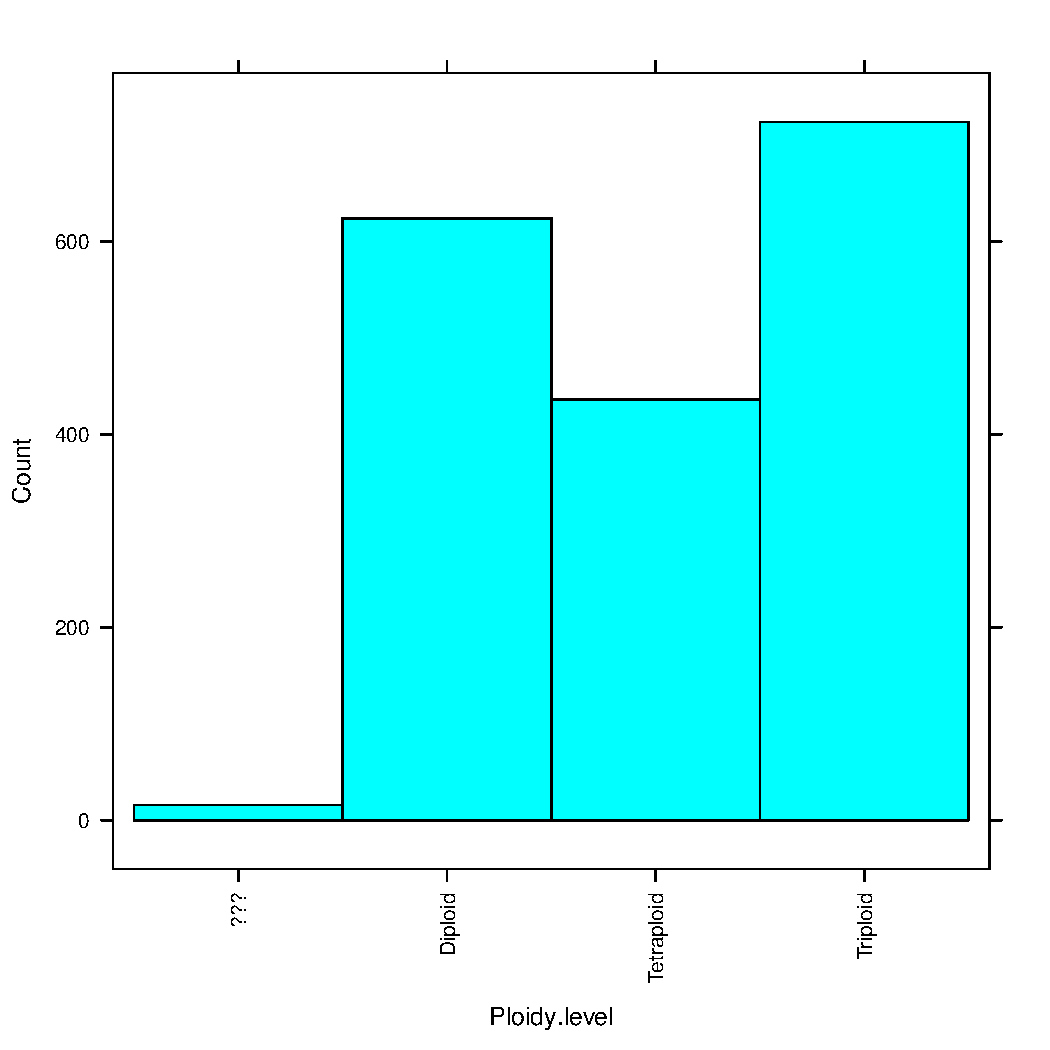
\includegraphics[width=\maxwidth]{figure/HistogramsPredictorVariables-6} 

}




{\centering 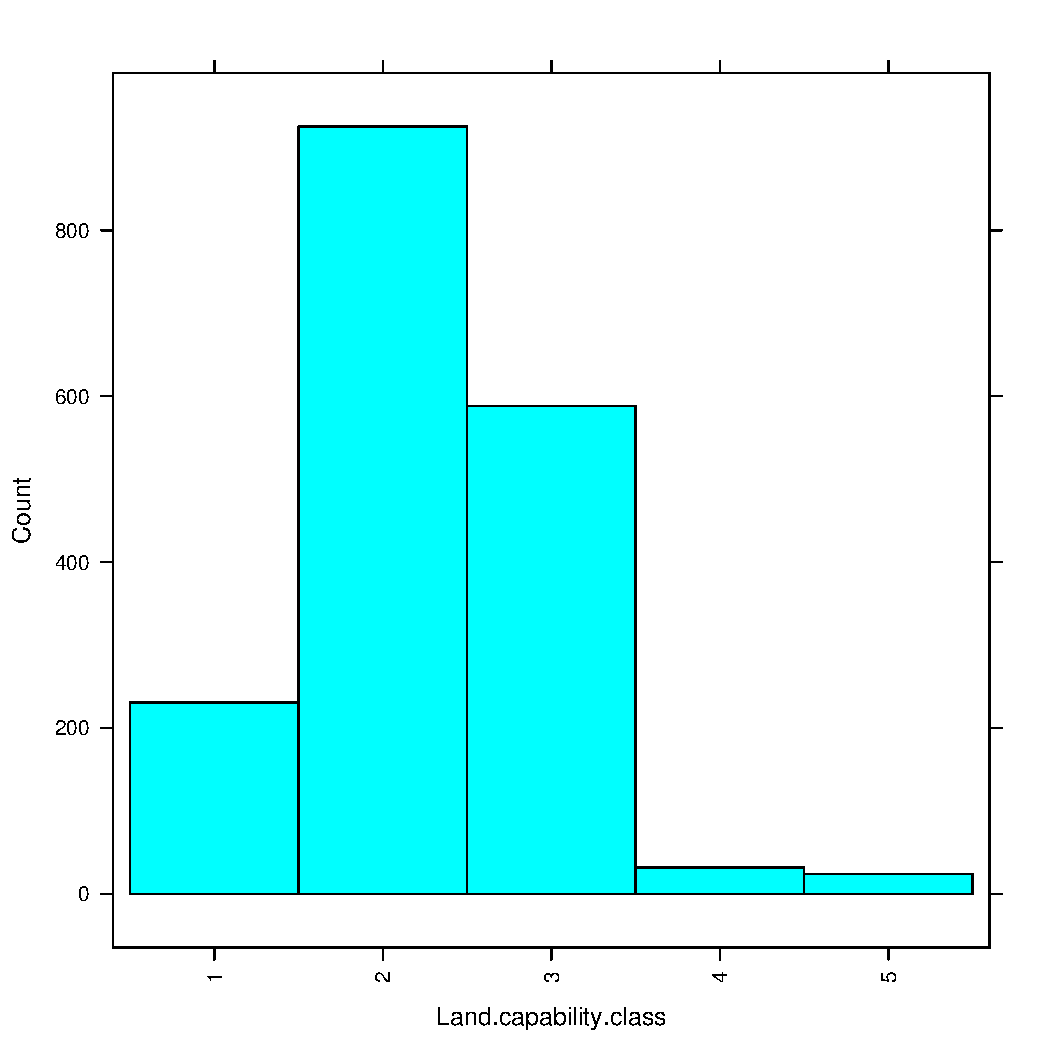
\includegraphics[width=\maxwidth]{figure/HistogramsPredictorVariables-7} 

}




{\centering 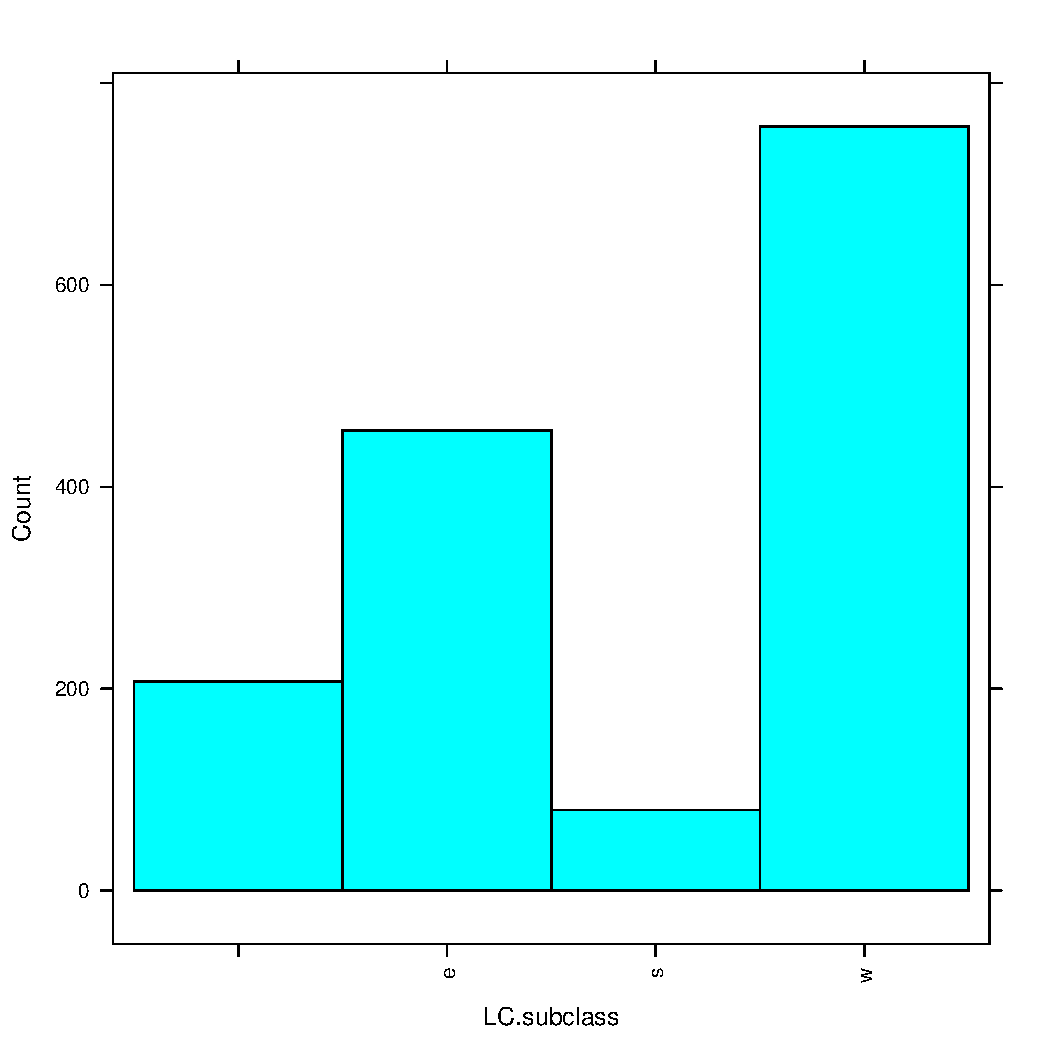
\includegraphics[width=\maxwidth]{figure/HistogramsPredictorVariables-8} 

}



\end{knitrout}

The histograms of the distribution of values in the Predictor group also indicate important aspects that need to be accounted for:
  
\begin{itemize}

  \item
  There are some clones that are represented with few data points and others that are represented with a large number of data points; the database is also biased with respect to clones.
  
  \item
  Clone, Epithet, Family, Diversity group are also unbalanced and are correlated. How do we handle the relationship between clone Epithet, Family, Diversity group? Also there are two Clone classifications, Clone ID and Clone Sas, which one do we use in the analysis? In particular the New Diversity group has entries 10, 13, 14, 15, 16, 3 with very few data points. There are clones with very few data points that are candidates to be excluded from the analysis.
  
  \item
  Ploidy level is also related to clone, family and Epithet, how do we manage the relationship with ploidy level? The level indicated by  question marks is one that was to be filled in the future? There are 
  16 
  labeled with question marks.
  Clone SAS 
  01X265020, 01X266016, 01X268016, 0X026083, 0X026084, 0X026085, 0X032095, 0X032096, 0X032097, 1X268017, 1X268018, 94006, 9882041, Dimitrios, India, Klara, Stina
  and Clone ID 
  94006, 9882-041, Dimitrios, India, Klara, Stina
   have 4 or less entries
  
  \item
  Land capability classes 4 (32) and 5 (24) have very few entries. Land capability class is related to site and land subclass.
          
  
  \item
  There are many variables that are correlated and we need to find a strategy to appropriately deal with the correlations. The first idea that comes to mind is to use a hierarchical method in the analysis. That is we start by only including location, then if location is important in explaining the variability we then replace location with variables related to location, to see which is the one that is important within location. A similar scheme could be used with the genotype variables.
  
  
\end{itemize} 

\subsubsection*{Genotype x Environment Distribution of Entries}

Using heat maps we can plot the number of entries across two variables simultaneously and that helps identify where the majority of entries or where the missing values are. For example by using a heat plot of the number of entries (counts) between Clone and location, we can easily see which locations have which clones and how many entries are per each clone.  A similar heat map can be plotted for ploidy level, family, epithet.

\begin{knitrout}
\definecolor{shadecolor}{rgb}{0.969, 0.969, 0.969}\color{fgcolor}

{\centering 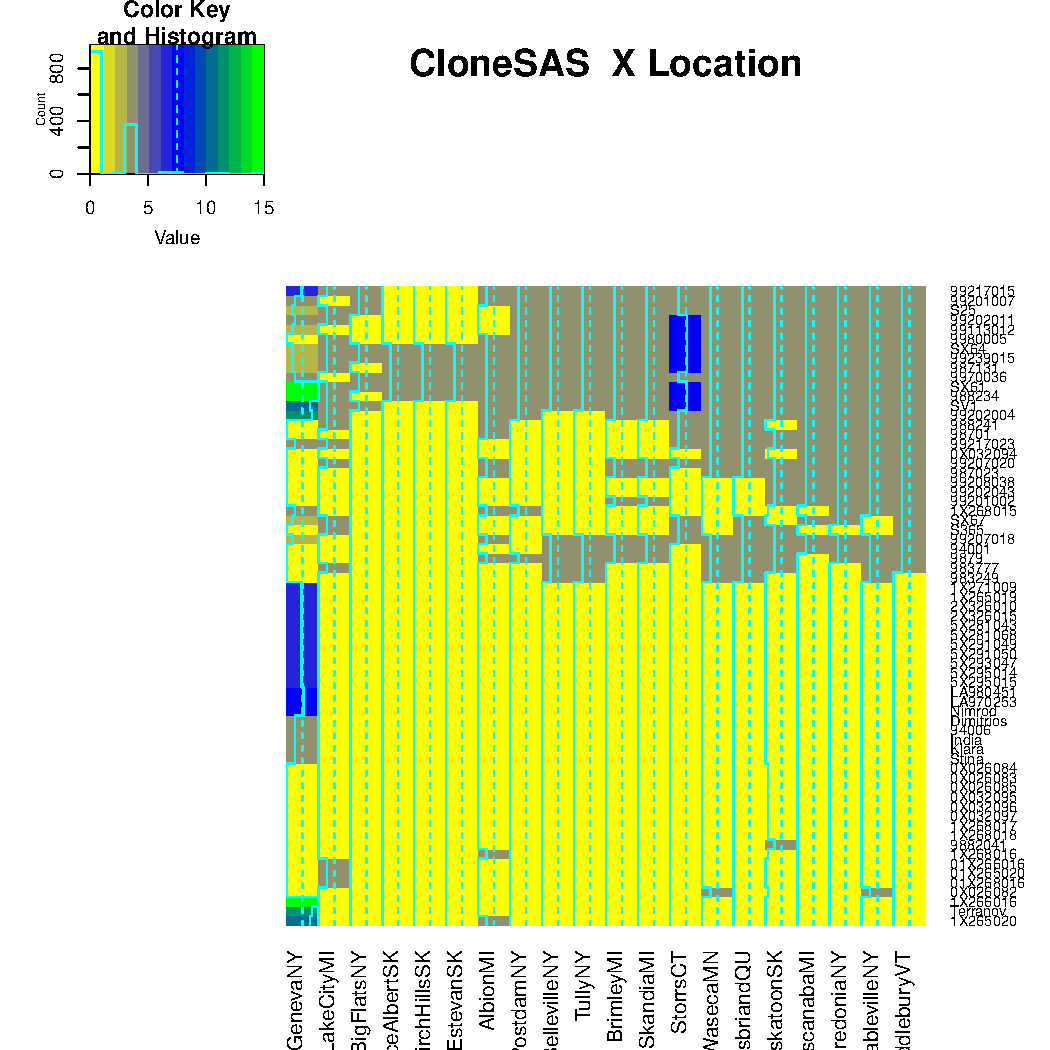
\includegraphics[width=\maxwidth]{figure/HeatmapCloneSASLocation-1} 

}




{\centering 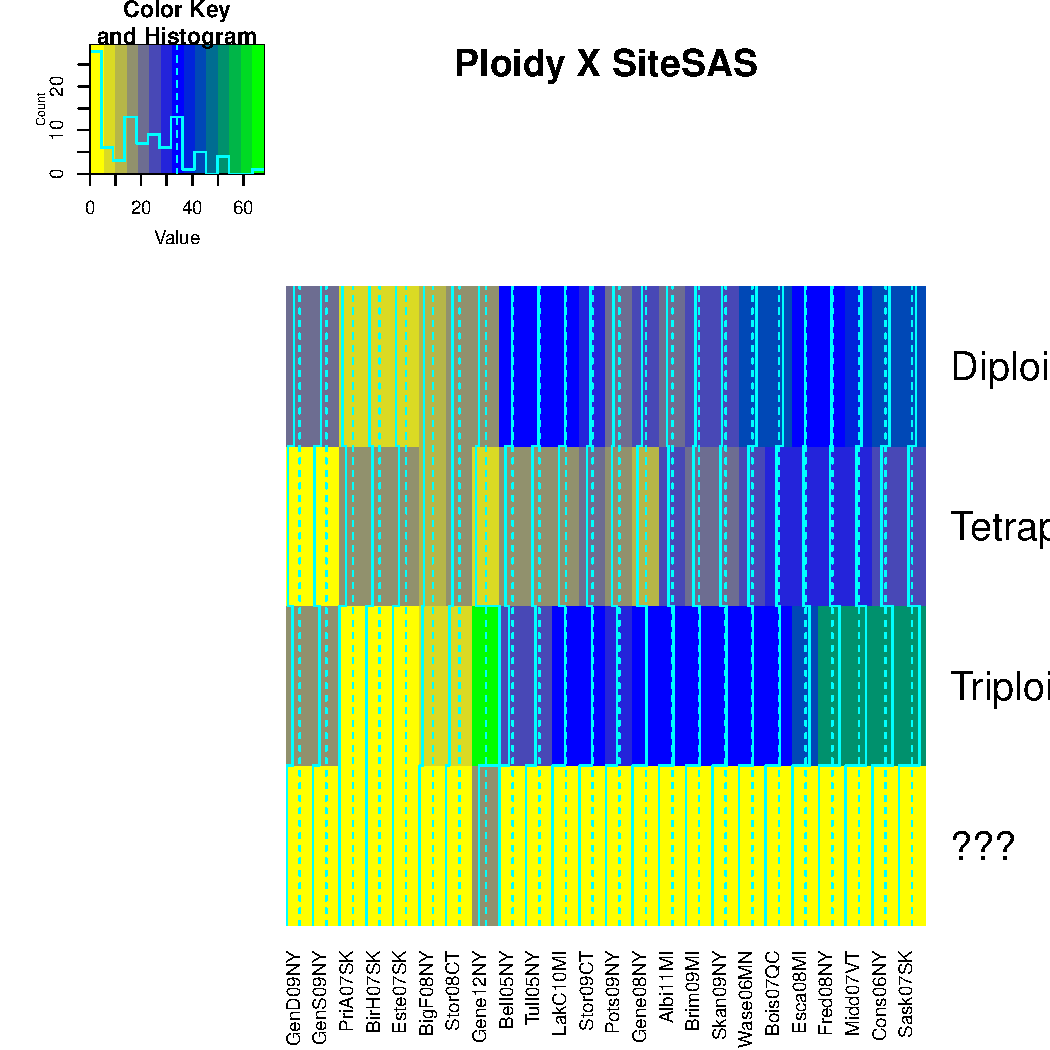
\includegraphics[width=\maxwidth]{figure/HeatmapCloneSASLocation-2} 

}




{\centering 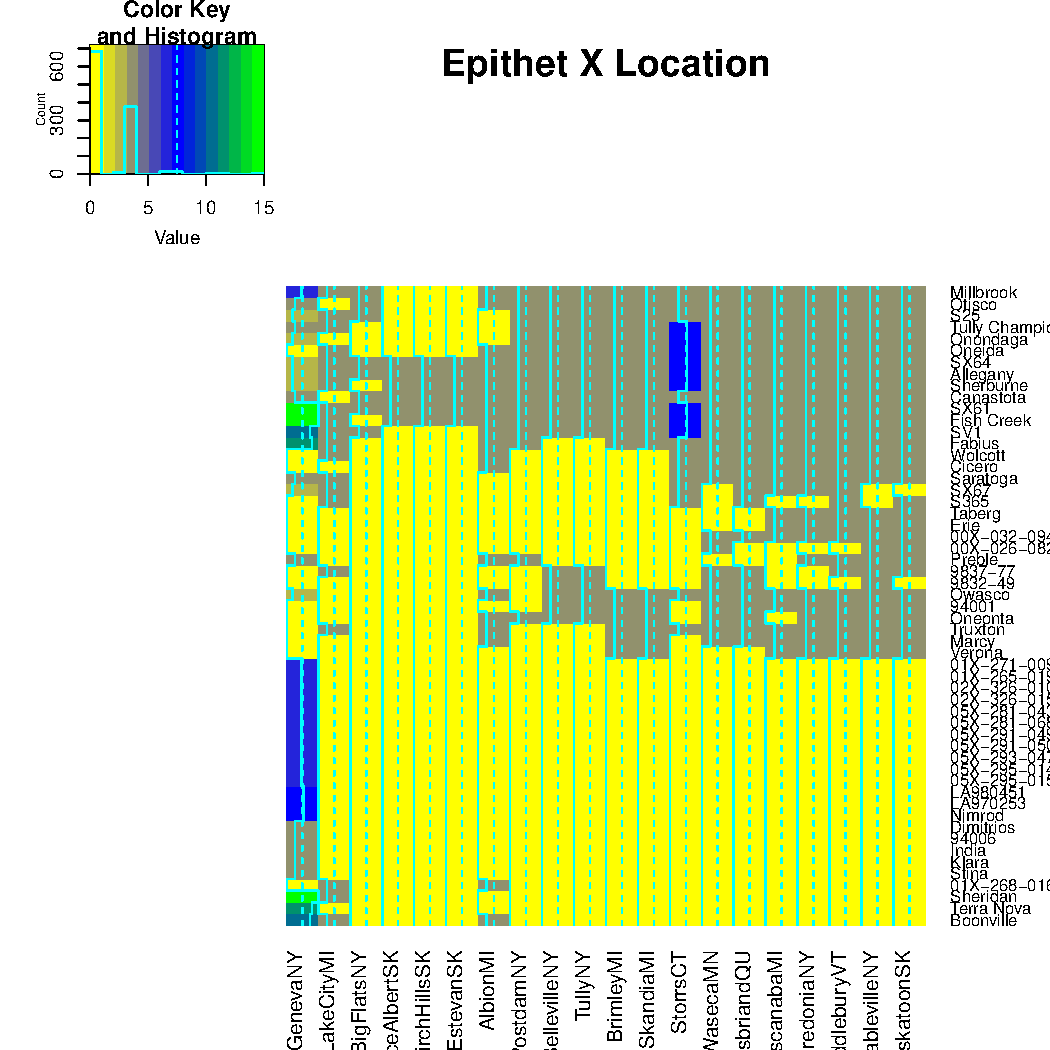
\includegraphics[width=\maxwidth]{figure/HeatmapCloneSASLocation-3} 

}




{\centering 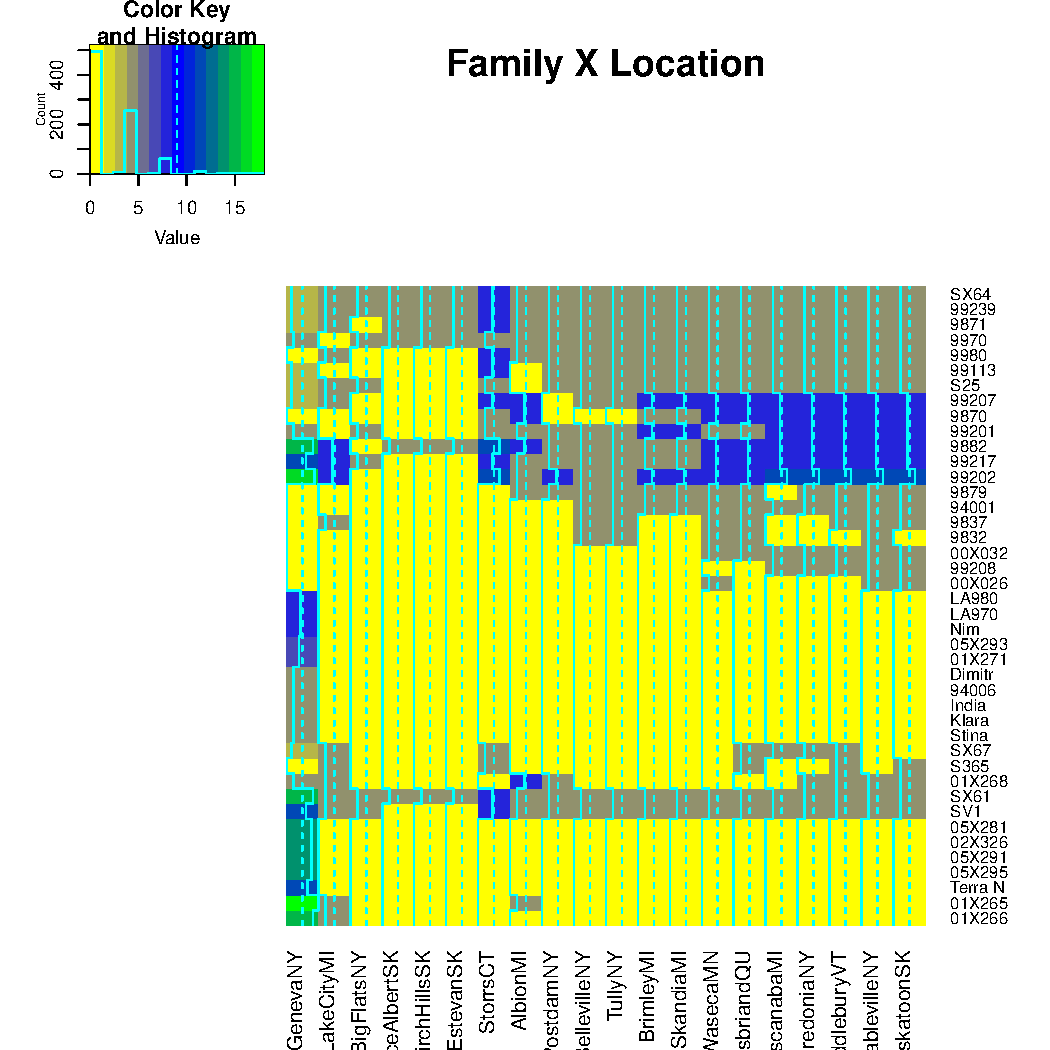
\includegraphics[width=\maxwidth]{figure/HeatmapCloneSASLocation-4} 

}



\end{knitrout}

\newpage
Using heat maps, abundance of data of different variables can also be explored. For example where is survival, yield, hemicellulose, diameter and height data is available and how many data entries are in each location. Should we leave out height and Od diameter since they have large gaps in the data? Should we keep Od Diameter since the gaps are distributed all over the locations?\\


\begin{knitrout}
\definecolor{shadecolor}{rgb}{0.969, 0.969, 0.969}\color{fgcolor}

{\centering 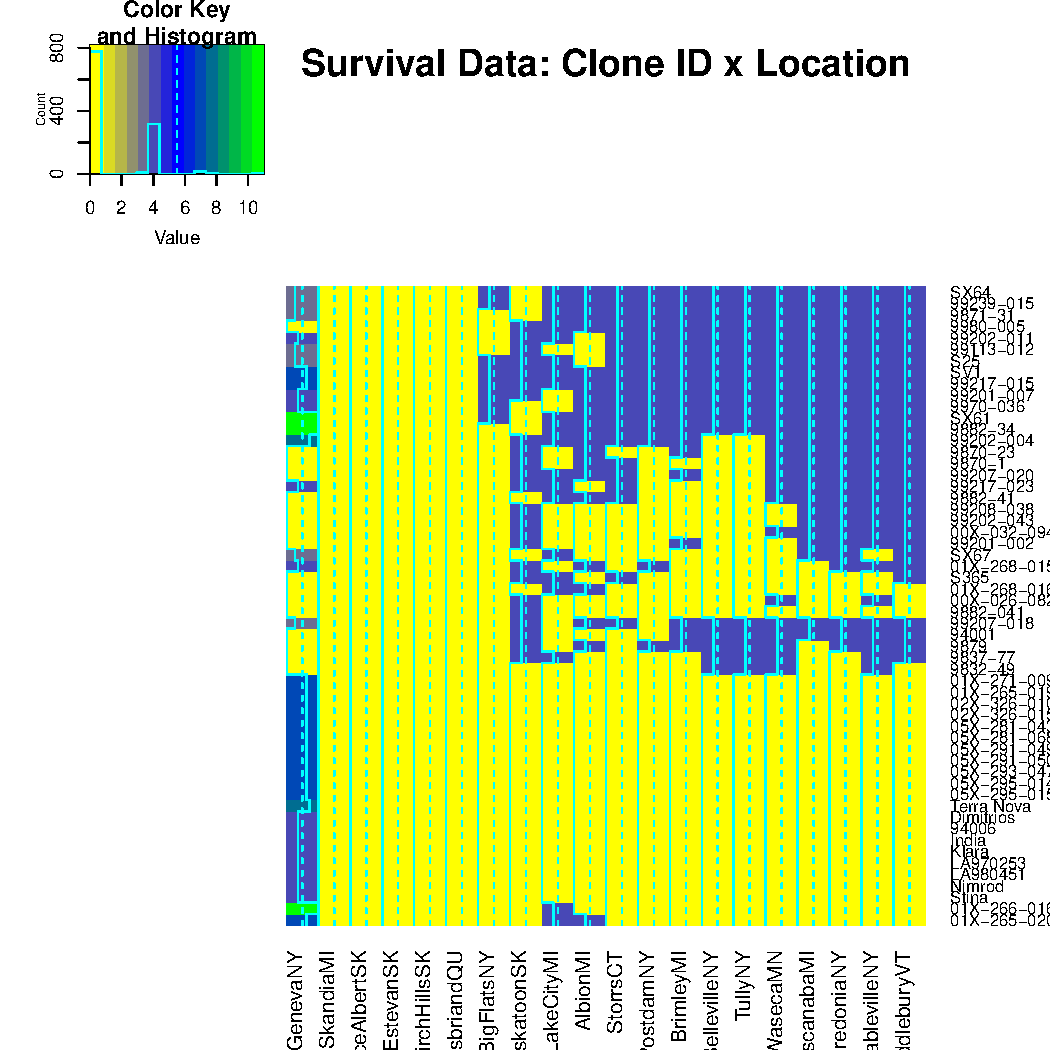
\includegraphics[width=\maxwidth]{figure/HeatmapSurvivalYield-1} 

}




{\centering 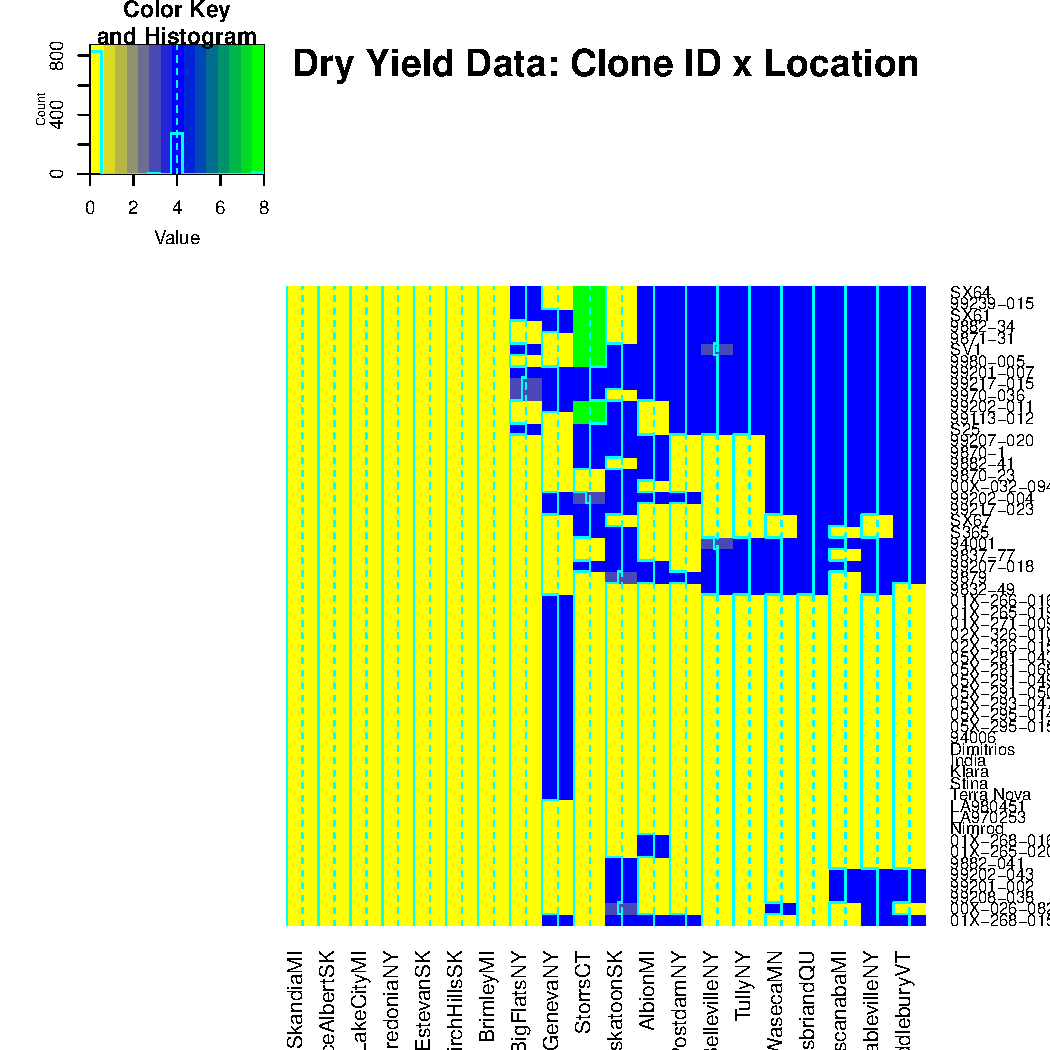
\includegraphics[width=\maxwidth]{figure/HeatmapSurvivalYield-2} 

}




{\centering 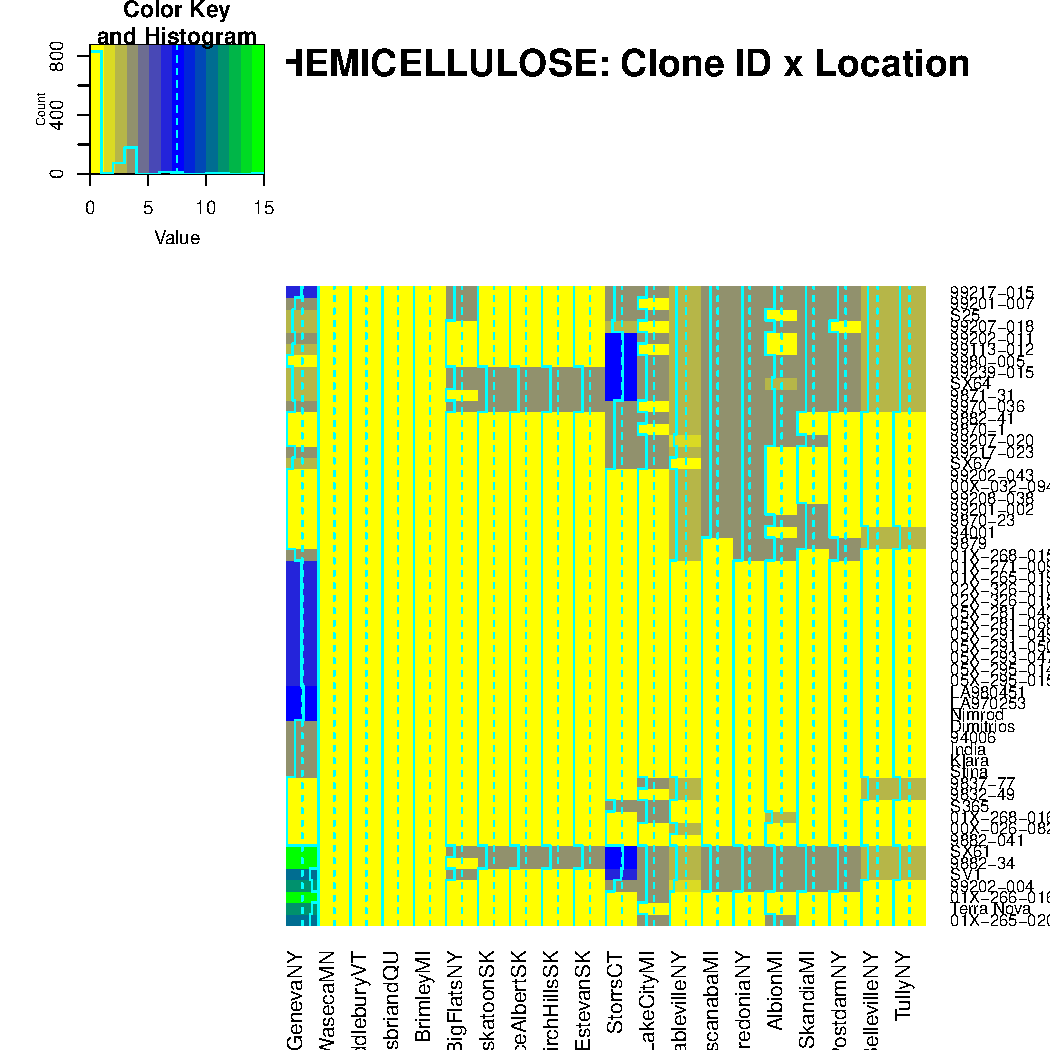
\includegraphics[width=\maxwidth]{figure/HeatmapSurvivalYield-3} 

}




{\centering 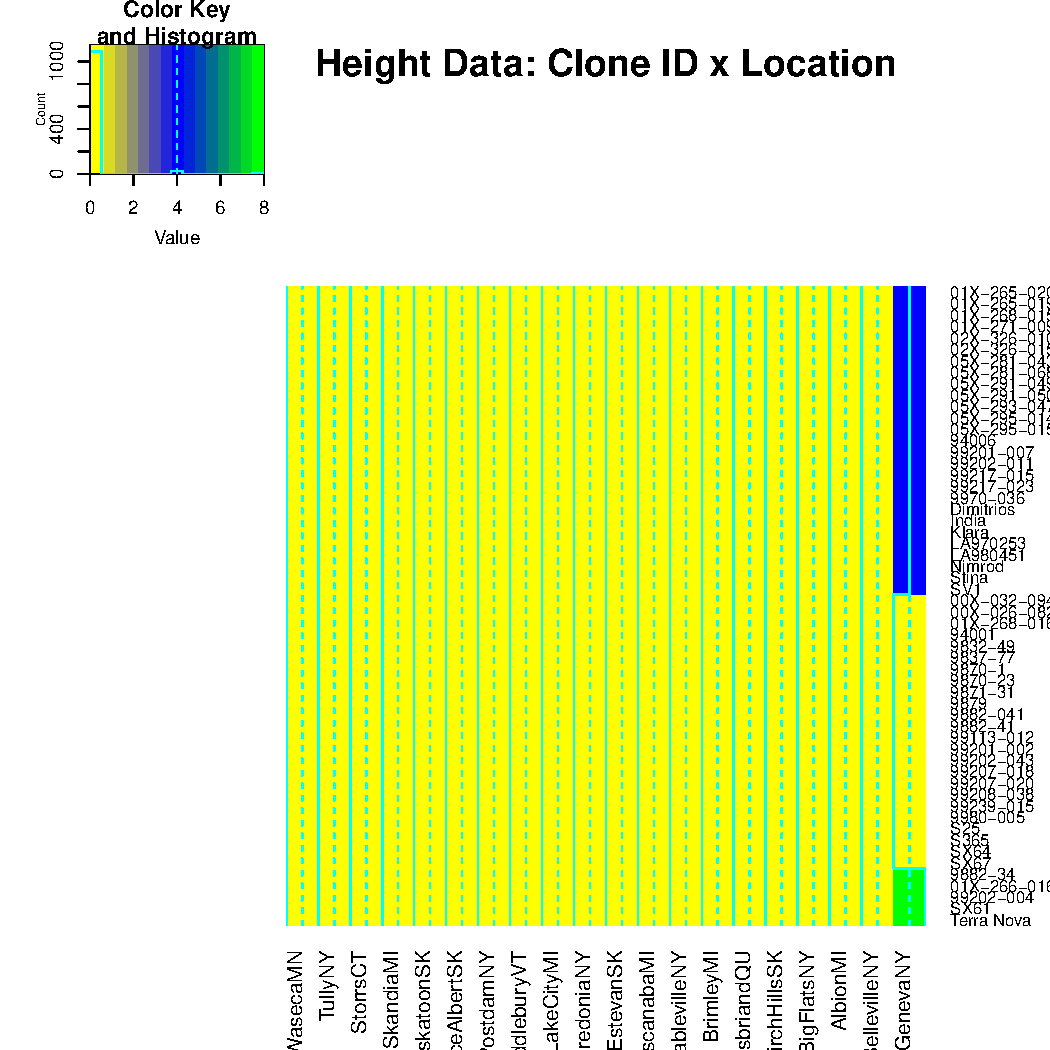
\includegraphics[width=\maxwidth]{figure/HeatmapSurvivalYield-4} 

}




{\centering 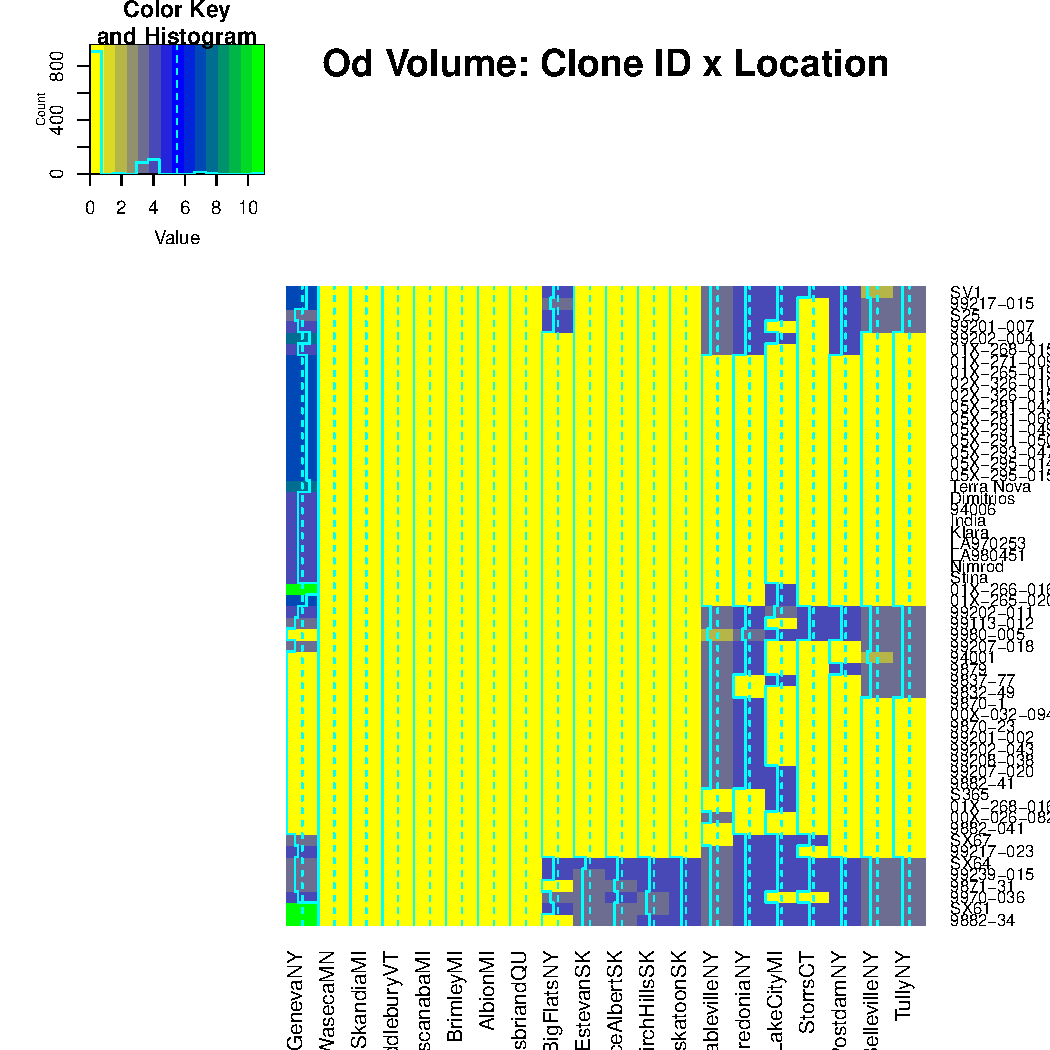
\includegraphics[width=\maxwidth]{figure/HeatmapSurvivalYield-5} 

}



\end{knitrout}


\section*{Random Forest Analysis}

\subsection*{Preliminaries}

Random forest analysis is very flexible in the assumptions it requires to complete a coherent analysis. There are a few requirements that the R package Random Forest impose on the analysis. The first one is that no response variable input is missing. That is if we are trying to predict biomass yield on using location, clone and weather, each data entry must have at least a value for biomass yield (the response variable) and some of the predictor variables clone, location and weather. The missing values of the predictor variables in a data entry can be estimated by the Random Forest algorithm, but the response variable needs to be present.
The second limitation of the Random Forest R Package is that it can only handle predictor variables that are factors with at most 53 levels. For example, if we have a predictor factor "location" that has 53 different values i.e. Geneva, Scanaba....53, the algorithm will run without a problem, but if the factor has 54 values, it will return an error. We might be able to circumvent this issue, but it might take time to investigate and resolve. In the mean time we can work with factors that have less than 53 levels and if they have more, we can get rid of the entries with levels that are not well represented or we can group these less represented levels into a group and carry the analysis with a reduced number of levels, but with all the data entries on it. This problem occurs with the predictor factor Clone ID or Clone SAS; there are more than 53 different clones in the database.\\

The strategy chosen to deal with the number of clones and be able to complete the Random Forest analysis, was to exclude from the analysis clones that had very few entries in the database. This strategy can be modified if needed, and if there are more ideas about it we should discuss them as we proceed. Based on the analysis describing the database the following clones had the fewest entries and were therefore excluded from the analysis: 
94006, 9882-041, Dimitrios, India, Klara, Stina. 
This brought the number of levels in the clone factor below 53 and therefore the analysis could be completed.\\

The simplest straight forward analysis that can be done is to take the database as is, with the reduced number of clones and apply the random forest analysis to it, without being concerned with correlations between variables, this would be the brute force approach.

\subsection*{Brute Force Approach}

Using the brute force approach with 500 trees, the random forest algorithm is able to explain 99.7\% of the variability in the data. At first glance this is impressive! A different conclusion emerges when the most important variables explaining the variation are tallied in a variance importance plot.\\


Number of trees: 500.\\

Number of variables tried at each split: 5.\\

Mean of squared residuals: 0.0316084. \\

\% Variability explained:  0.9977047.\\



\begin{knitrout}
\definecolor{shadecolor}{rgb}{0.969, 0.969, 0.969}\color{fgcolor}

{\centering 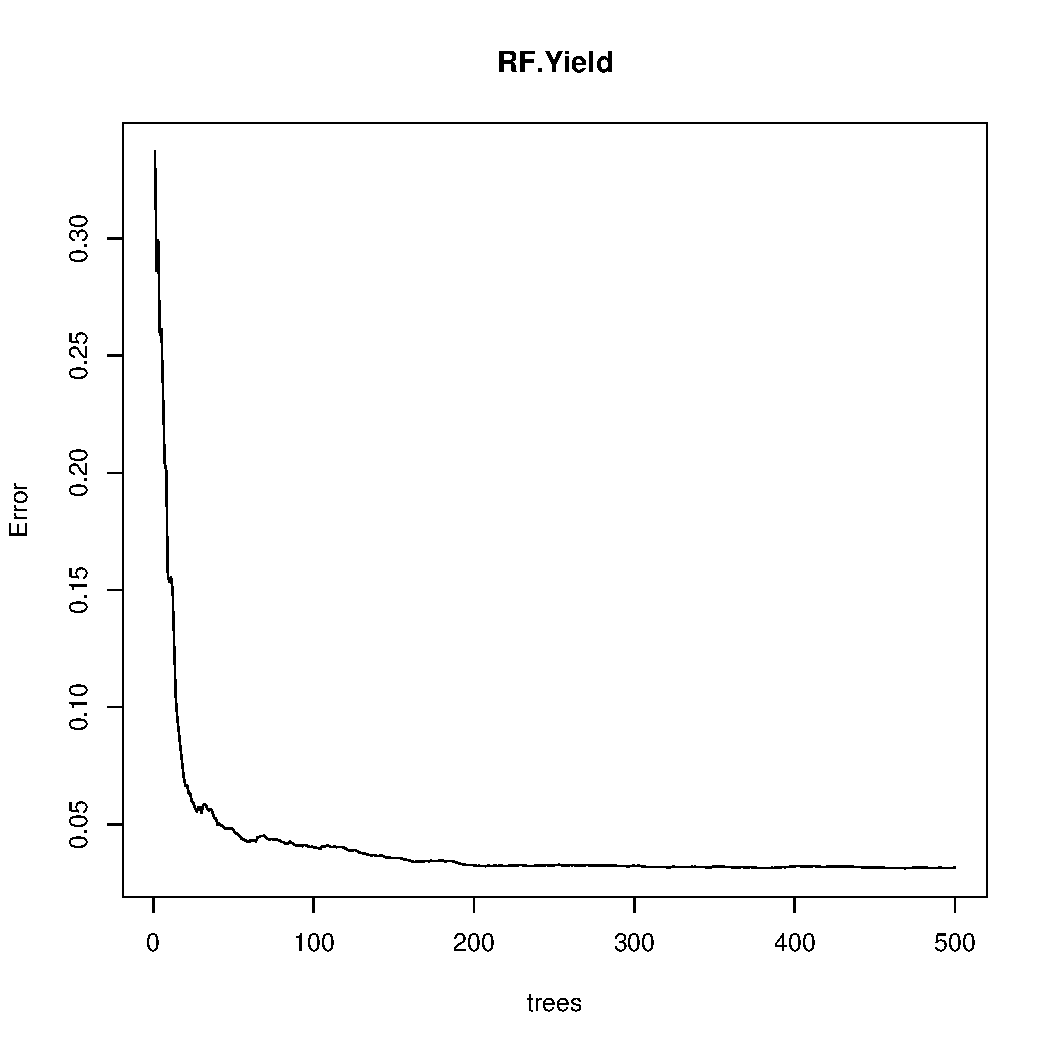
\includegraphics[width=\maxwidth]{figure/BruteForceApproach-1} 

}




{\centering 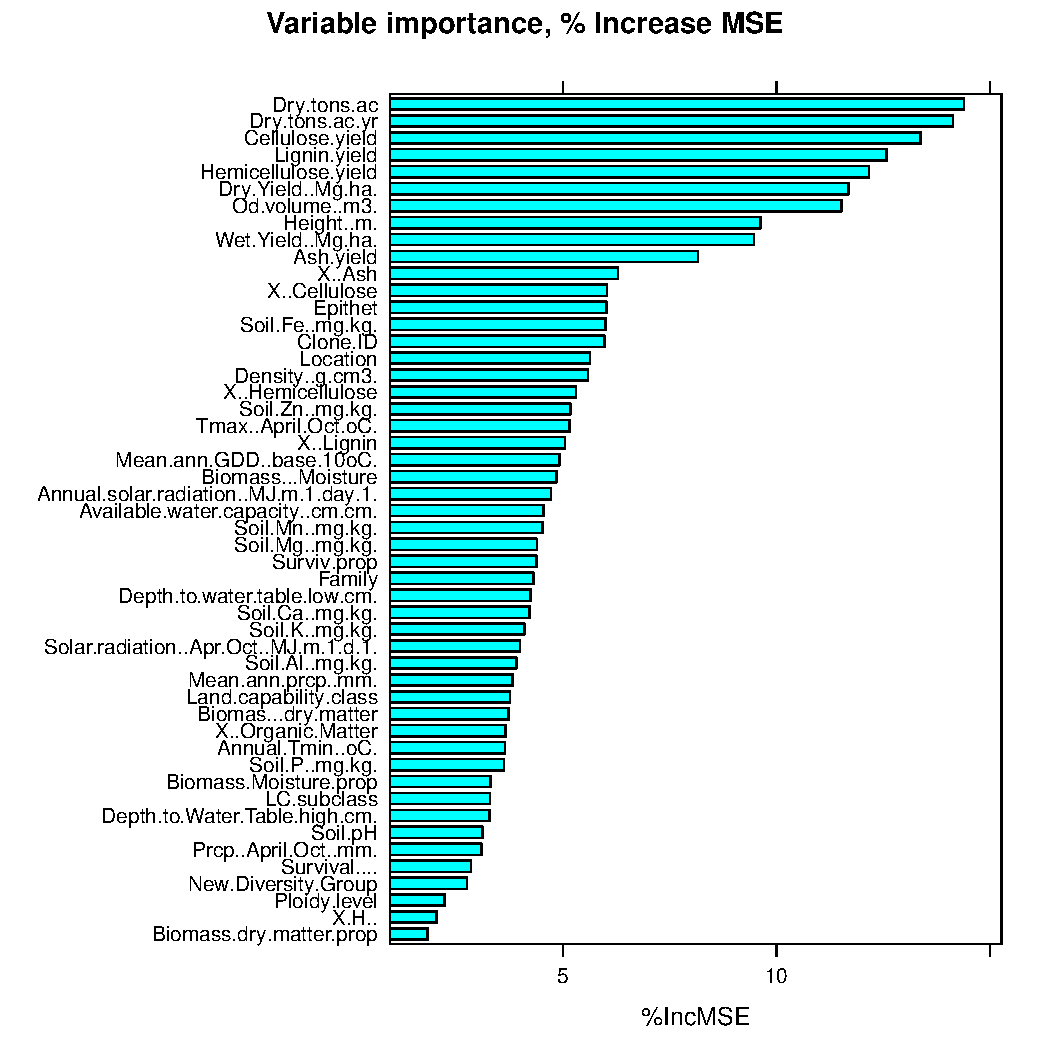
\includegraphics[width=\maxwidth]{figure/BruteForceApproach-2} 

}




{\centering 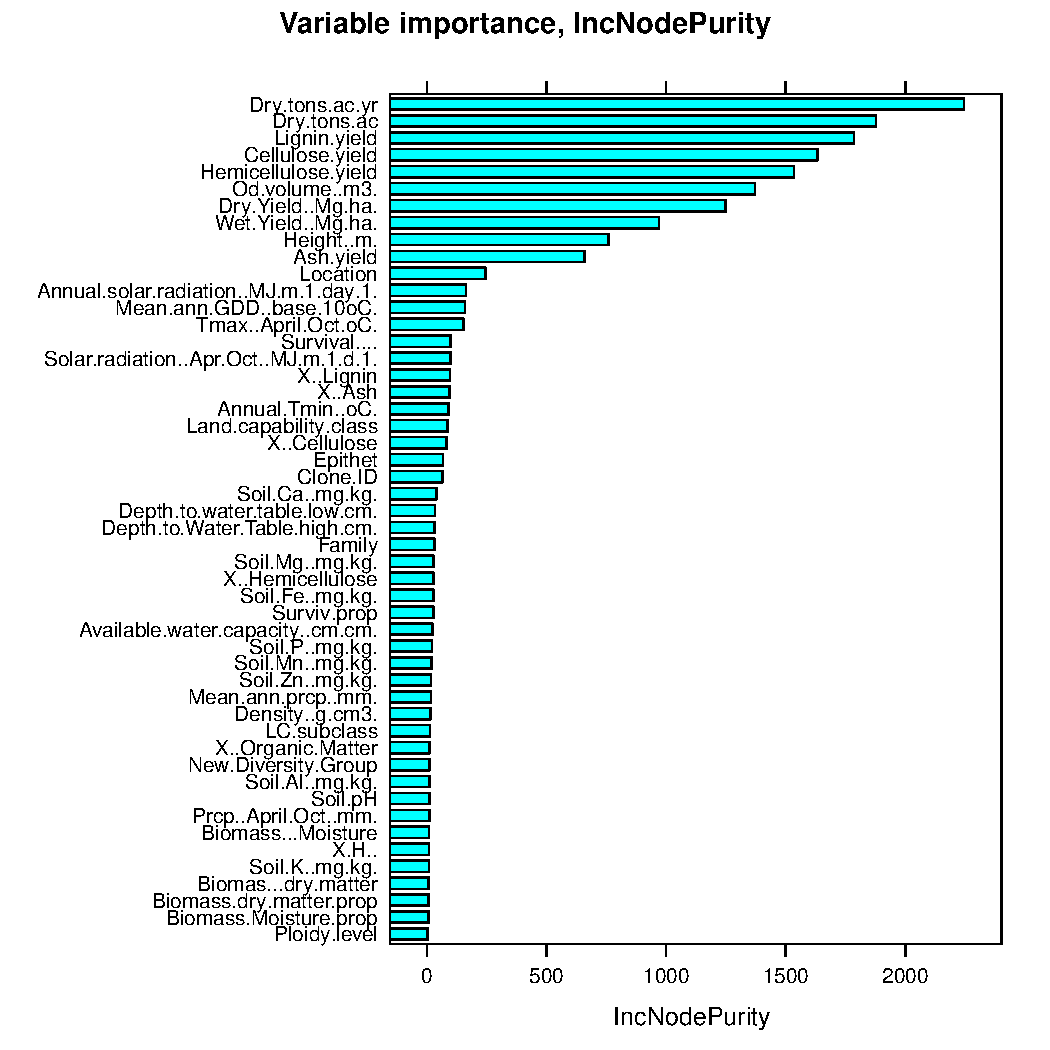
\includegraphics[width=\maxwidth]{figure/BruteForceApproach-3} 

}



\end{knitrout}


Doing blindly the random forest procedure is a bad idea as it can be seen in the figure generated above. There are many variables that are related to each other and make no sense in answering scientific questions, but are great for predicting the response to yield. The initial random forest results with all variables explaining yield, indicated that obviously correlated variables (wet yield, ash yield, ligning yield, OD Volume, height) were the most important. Variables that have large gaps in the data, height and OD diameter, appear as important predictors of yield because of the imputed process for missing data and their high correlation with yield. This is not unexpected but for sure is of no use. A more useful result would be obtained when these correlated variables are not included in the analysis. Also, since location determines, soil  pH, and all the other soil variables, all those variables are correlated and should not be at the same time in the analysis.

\subsection*{Initial variable Selection approach}

Compared to the brute force approach illustrated in the previous section, a more efficient and instructive approach is to select variables that are believed to be important to answer the scientific questions asked of the data and try the analysis with those variables. Repeating the process of selected scientific questions and the variables that may be responsible for the answers and performing the random forest analysis on them, if done strategically and in a thoughtful manner would indicate which variables or factors are responsible for a particular response.
Here is where Larry, Armen and Eric's input would be essential.\\

Identifying the main variables and factors determining yield is the first question that is going to be analyzed following the method described above. The analysis was based on my (Felipe) subjective selection of variables and can be changed with minor effort to a different selection of variables if a better selection is suggested. Also, the data was used with the reduced clone numbers explained above, and with missing data in the predictor values imputed using the complete database  with the Random Forest impute procedure; this step can also be modified easily if a subset of the database is chosen to be more appropriate.\\

Variable Annual Yield (Mg/ha/yr) was explained using the following predictor variables: "Mean.ann.prcp..mm." , "Mean.ann.GDD..base.10oC." , "Prcp..April.Oct..mm." ,  "Tmax..April.Oct.oC." , "Annual.Tmin..oC." , "Annual.solar.radiation..MJ.m.1.day.1.", "Solar.radiation..Apr.Oct..MJ.m.1.d.1." , "Depth.to.water.table.low.cm." , "Depth.to.Water.Table.high.cm." , "Available.water.capacity..cm.cm.", "Survival...." , "Biomass...Moisture" , "Biomas...dry.matter" , "X..Hemicellulose" , "X..Cellulose" , "X..Lignin" , "X..Ash" , "Density..g.cm3." , "Location" , "Clone.ID" , "Epithet" , "Family" , "New.Diversity.Group" and "Ploidy.level". The names of the variables are not exactly as they appear in the original database because the way they are encoded in R when read from a MS Excel spreadsheet, but that can be changed easily if needed; in the mean time the current names have a direct representation of the names in the original data base. When carried out the Random Forest analysis as indicated above, the following results are obtained:

Number of trees: 500.\\

Number of variables tried at each split: 5.\\

Mean of squared residuals: 3.381958. \\

\% Variability explained:  0.7544096.\\ 

The reduced number of variables resulted in an increase in the mean squared of the residuals from 0.0316084  to  3.381958 and a decrease in percent variability explained from  0.9977047   to    0.7544096.
The set of predictor variables used in the analysis is still not optimum and have variables that are still highly correlated; it can be improved for sure. Nonetheless it shows major differences with the brute force approach. Looking at the tallies of the variable importance in the figures below, location and environmental variables become more important. Other variables that increase importance are family, epithet, survival, Clone ID, composition variables such as Fraction of Lingnin (X..Linging in the chart) and the fraction of cellulose (X..Cellulose). \\


\begin{knitrout}
\definecolor{shadecolor}{rgb}{0.969, 0.969, 0.969}\color{fgcolor}

{\centering 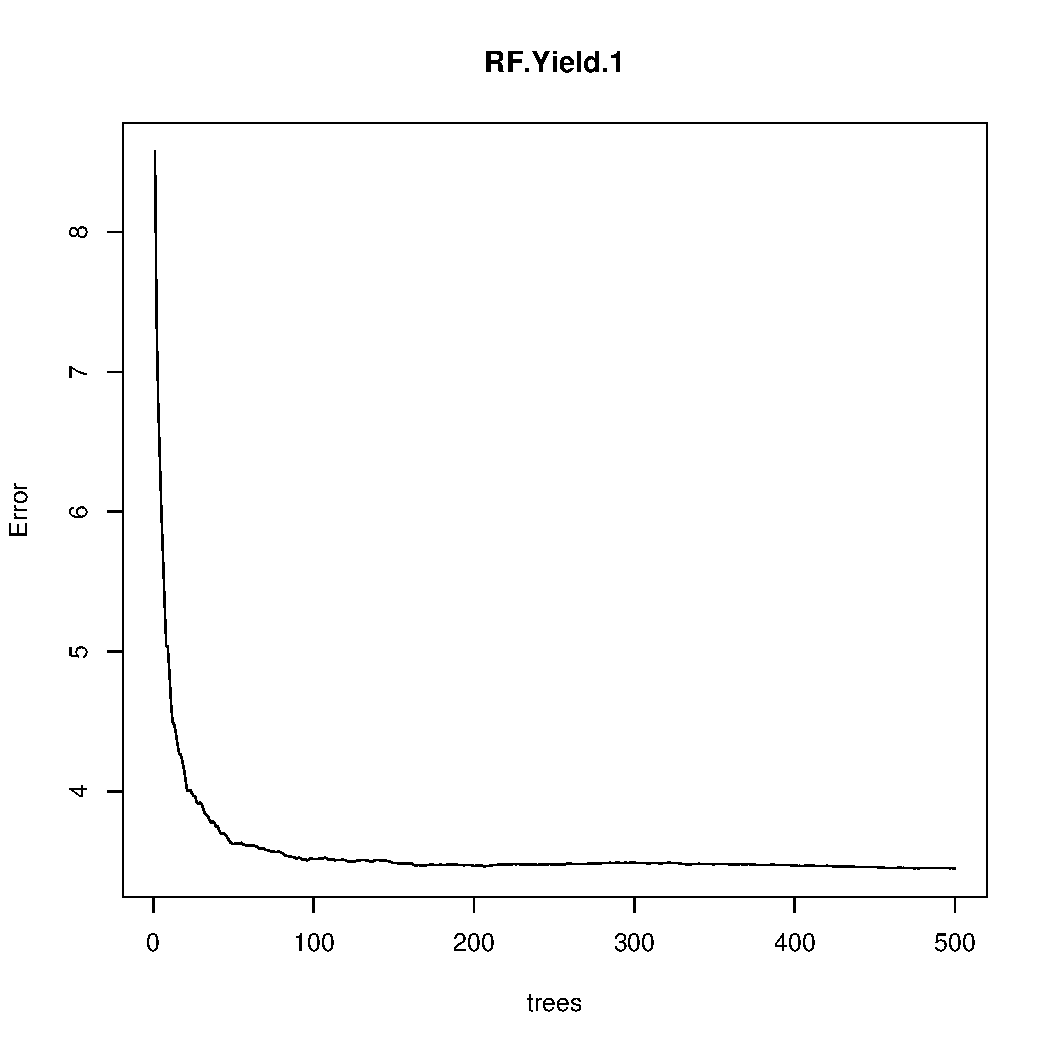
\includegraphics[width=\maxwidth]{figure/VariableSelectionApproach-1} 

}




{\centering 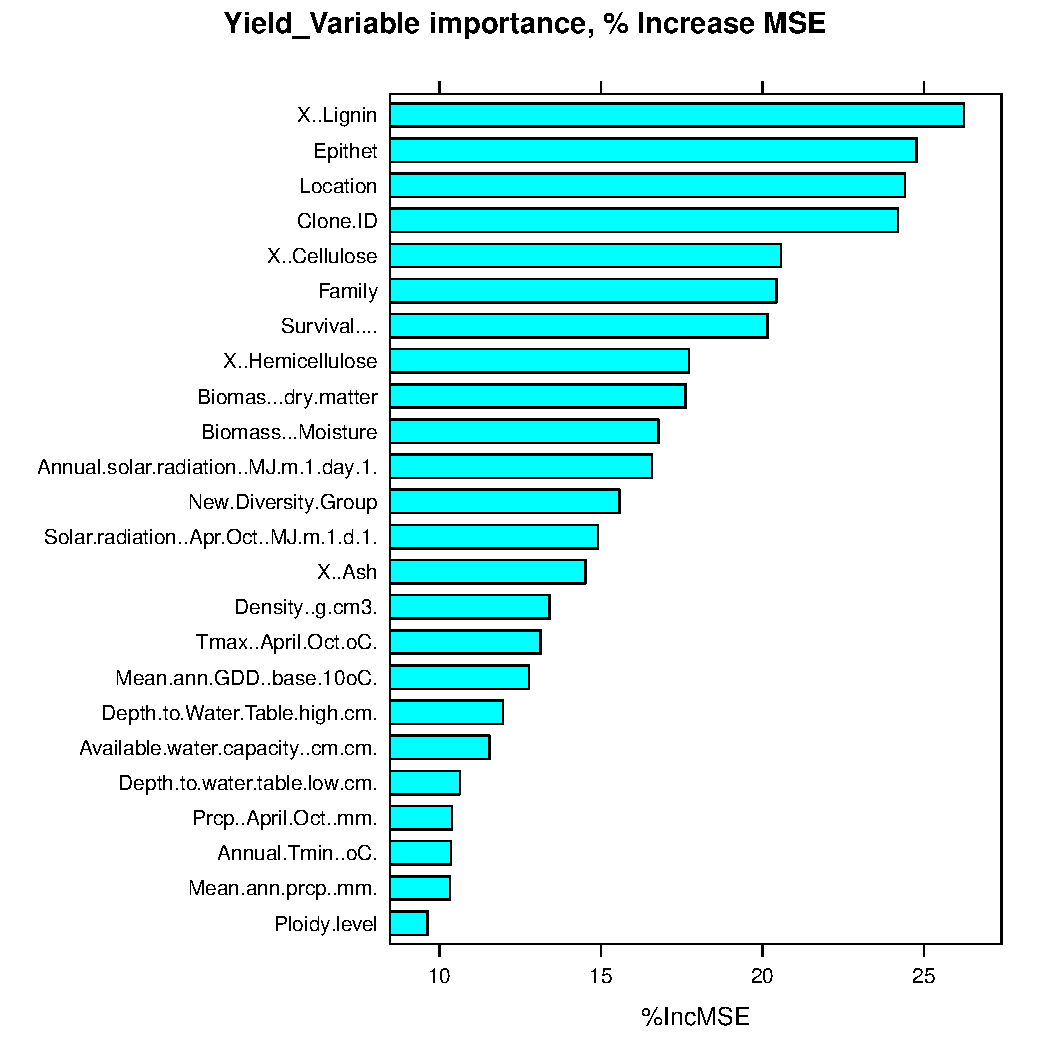
\includegraphics[width=\maxwidth]{figure/VariableSelectionApproach-2} 

}




{\centering 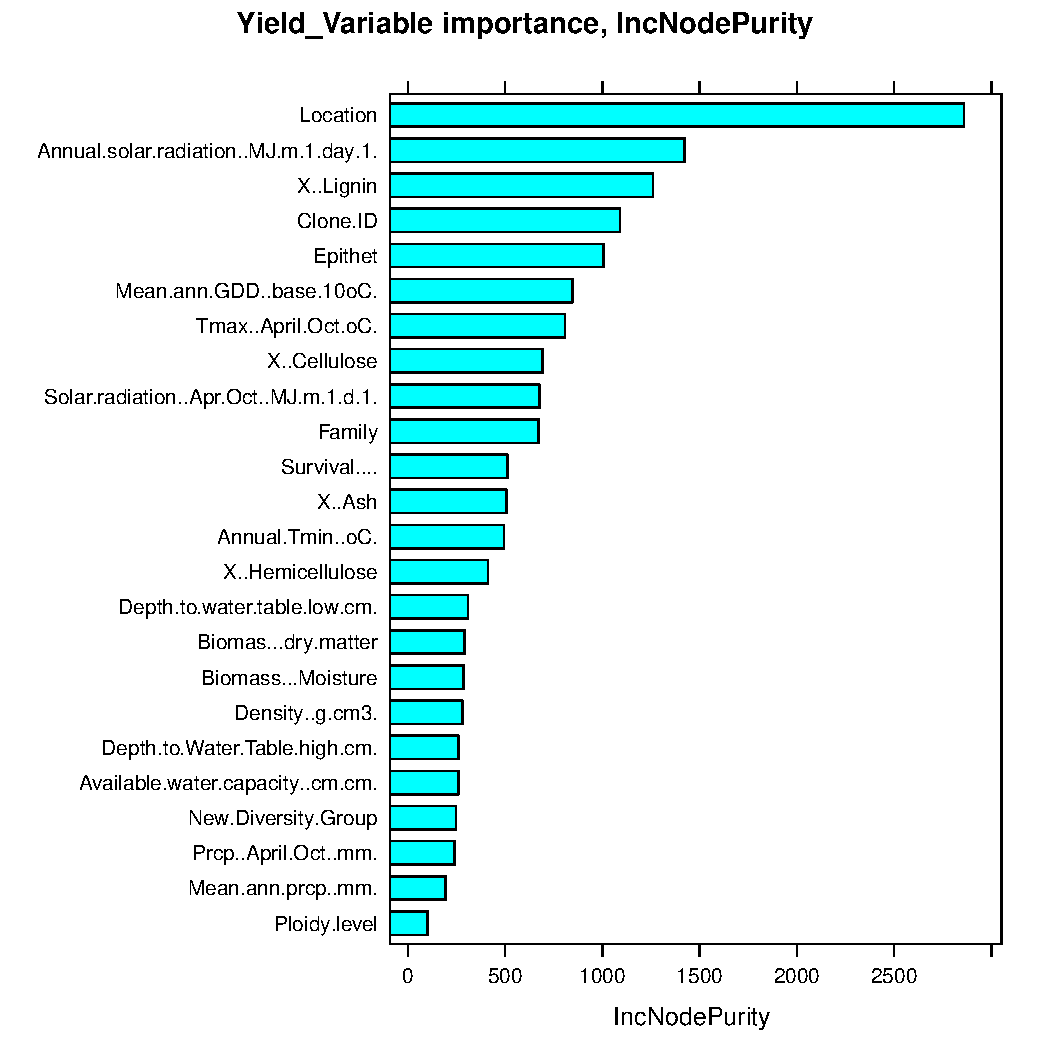
\includegraphics[width=\maxwidth]{figure/VariableSelectionApproach-3} 

}



\end{knitrout}
\\

It is possible to look to the role each variable plays in explaining variability by the partial dependence of the response variable to each predictor variable. The partial dependence analysis indicate the predictive value of each level of a particular predictor when all the other predictors varied randomly. This is easier to illustrate with an example. Plotting the partial dependence of yield to each level of the factor "Location" results in the following relationship:\\



\begin{knitrout}
\definecolor{shadecolor}{rgb}{0.969, 0.969, 0.969}\color{fgcolor}

{\centering 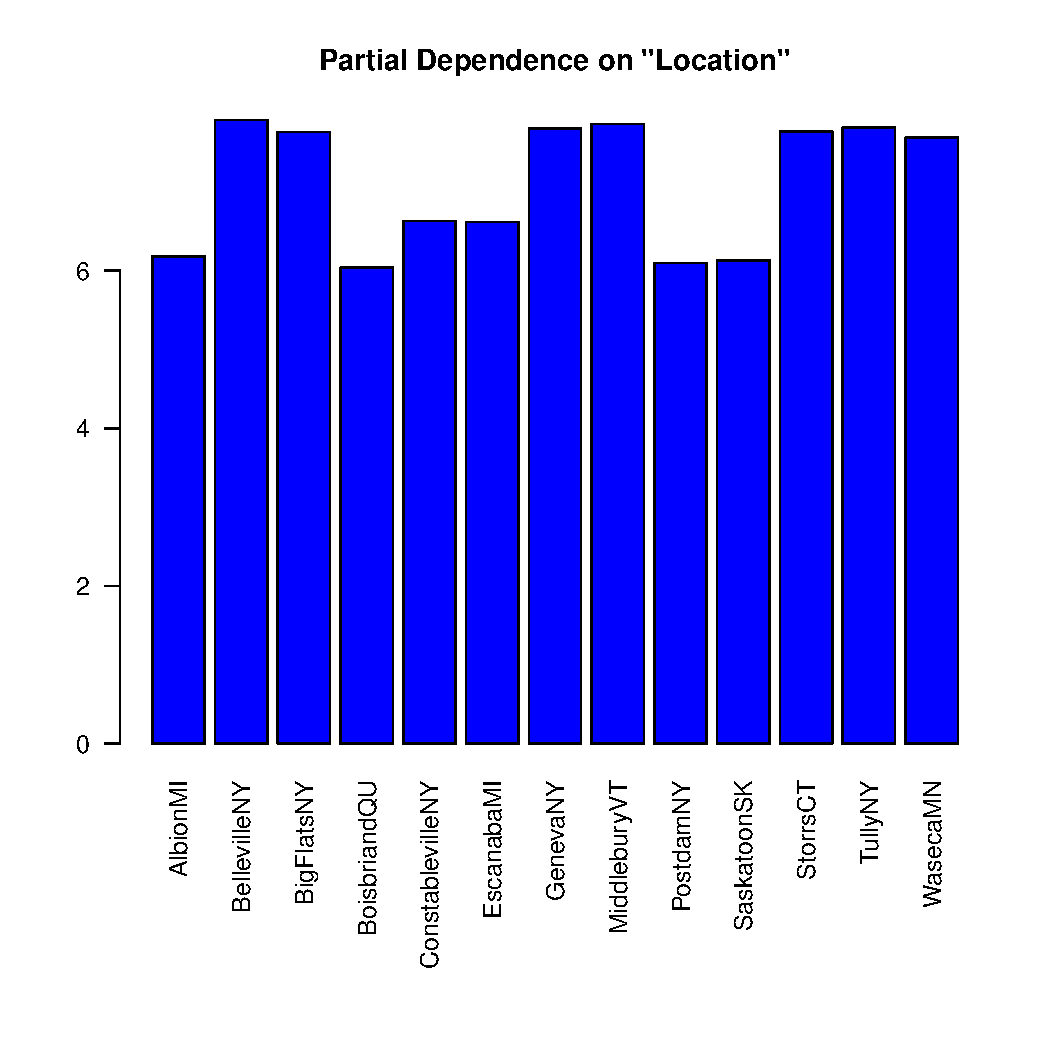
\includegraphics[width=\maxwidth]{figure/PartialDependenceLocation-1} 

}



\end{knitrout}

In the partial dependence plot of yield vs location is difficult to see any particular increase in prediction related to a particular level of the factor "Location". That is, there is no Location that have more predictive power over the others; some have a little higher prediction power than others, but there is not a clear trend. Contrast the previous graph with the partial dependence plot of yield vs Lignin content (X..Lignin); there is an  important change in the relation ship between yield and lignin content and it is nonlinear. As ligning content changes from 24\% to 26\%  the relationship between yield and ligning content changes significantly, even when all the other variables change randomly.
Therefore, lignin content is an important predictor of yield: no surprise here! In similar way but in opposite direction, the relationship between yield and cellulose content (X..Cellulose) between 40\% to 45\% changed significantly; increasing cellulose content from 40\% to 45\% has an important increase in the prediction of yield. The same analysis can be applied to partial dependence of yield to survival, clone, epithet and ploidy level, to name some of the important variables.  


\begin{knitrout}
\definecolor{shadecolor}{rgb}{0.969, 0.969, 0.969}\color{fgcolor}

{\centering 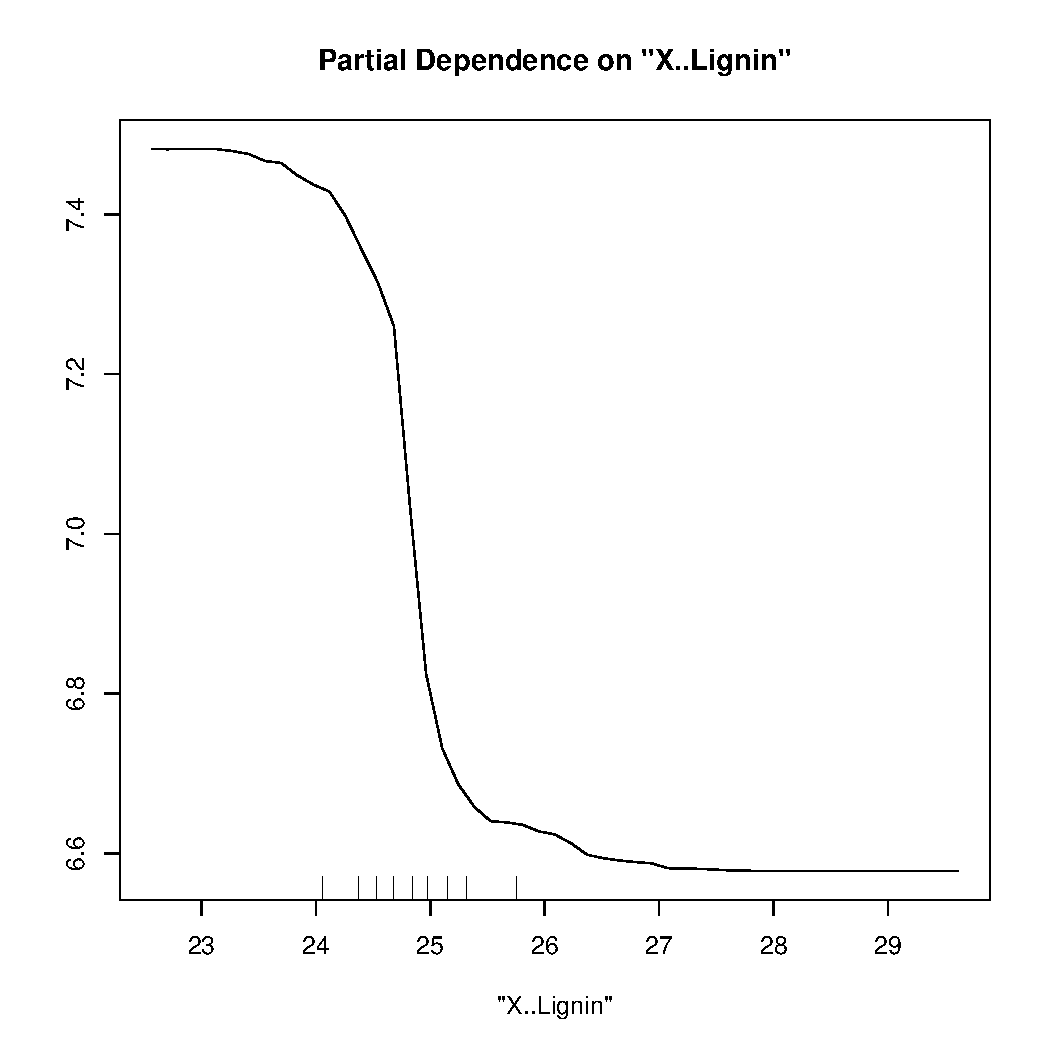
\includegraphics[width=\maxwidth]{figure/PartialDependence-1} 

}




{\centering 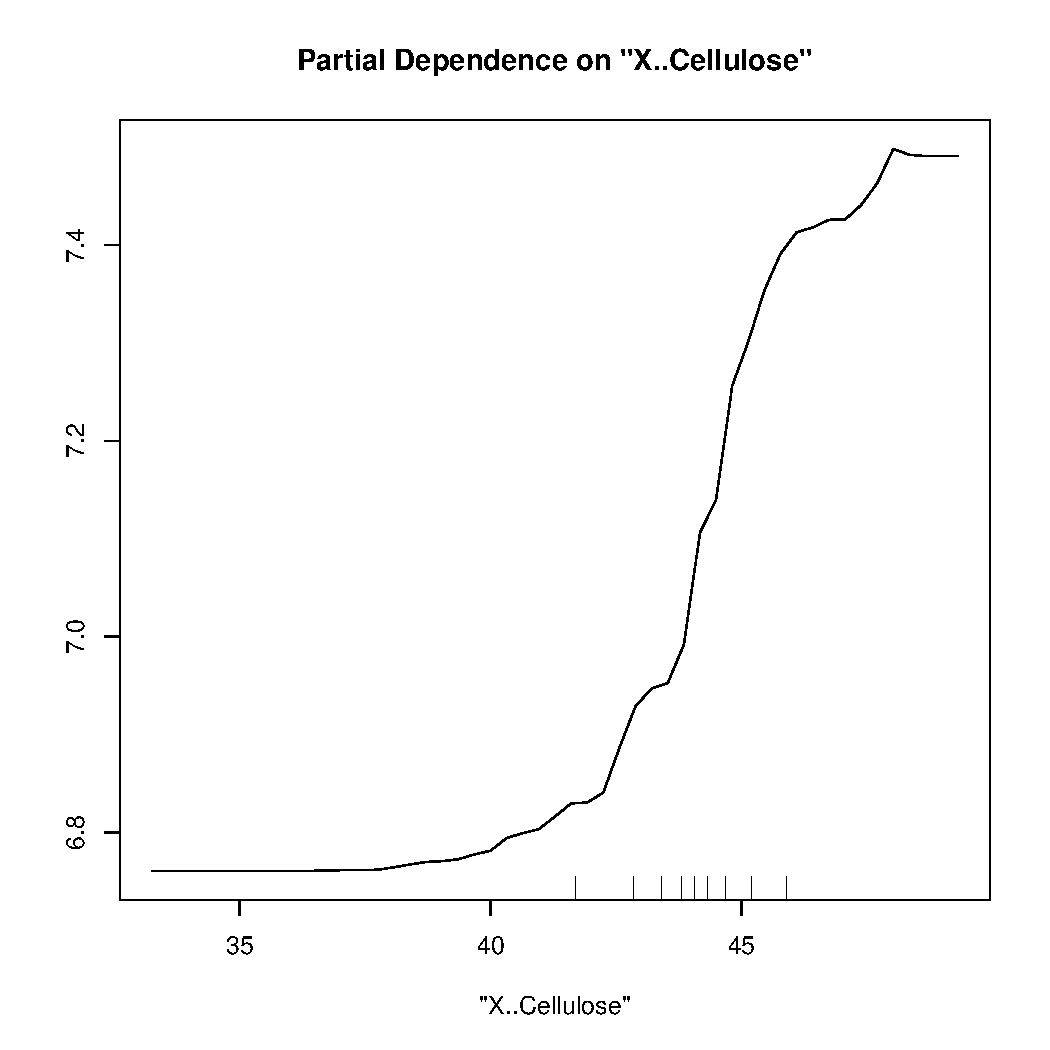
\includegraphics[width=\maxwidth]{figure/PartialDependence-2} 

}




{\centering 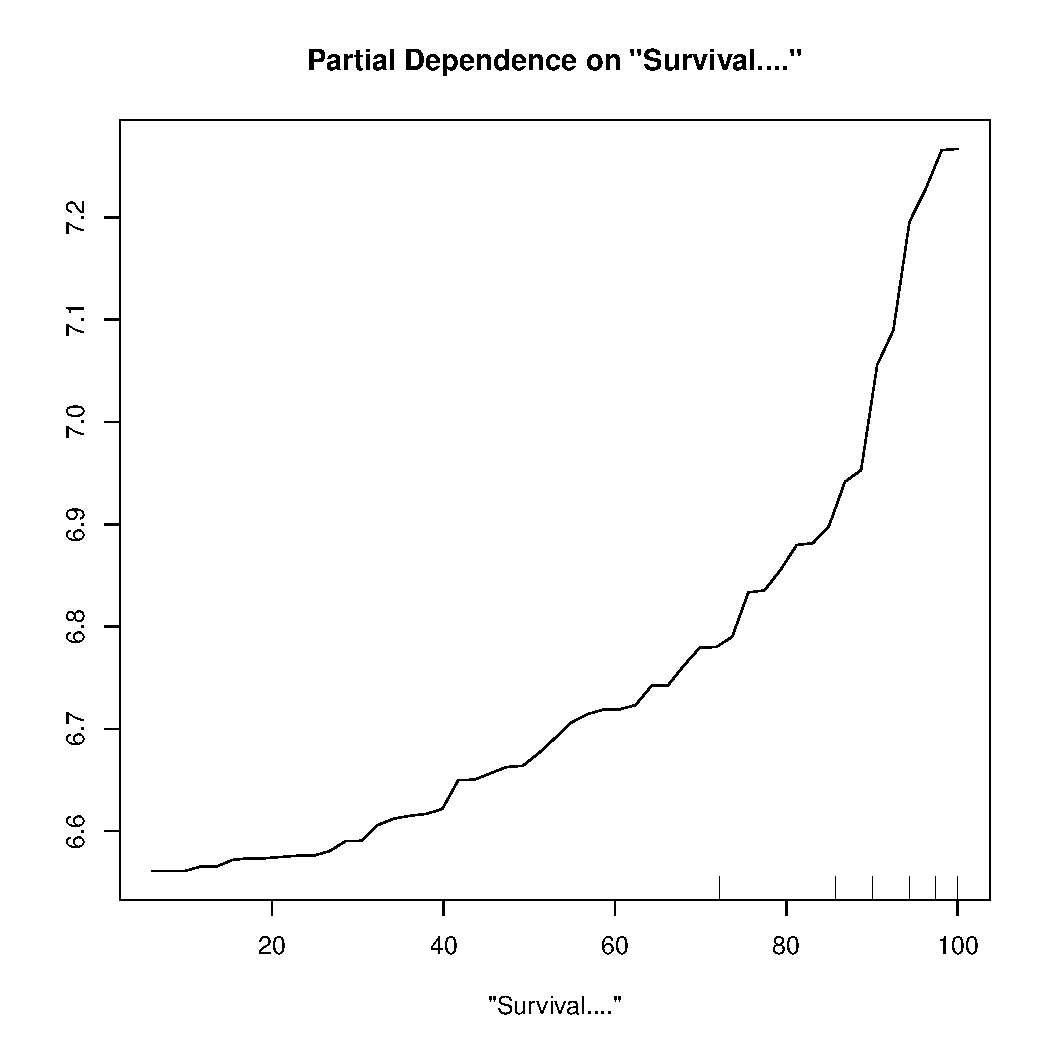
\includegraphics[width=\maxwidth]{figure/PartialDependence-3} 

}




{\centering 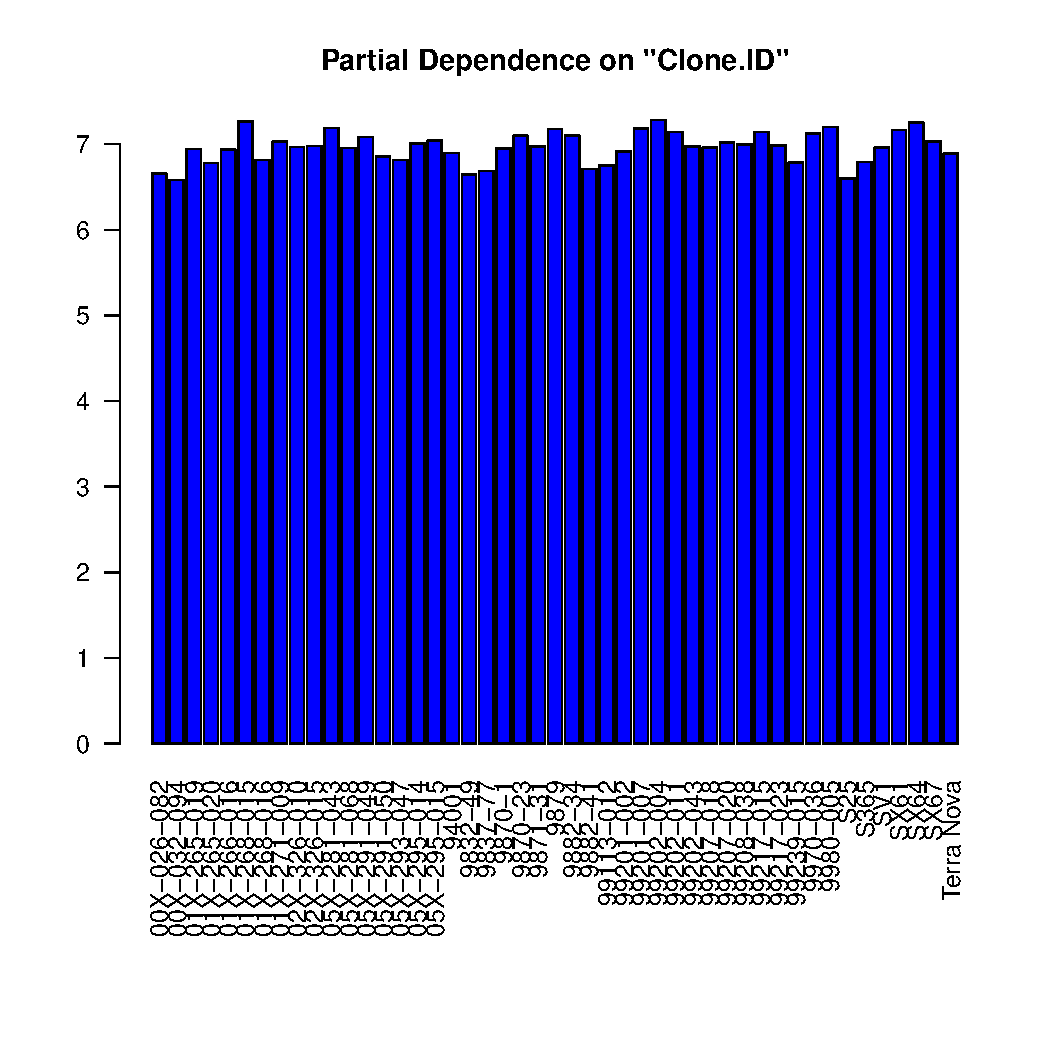
\includegraphics[width=\maxwidth]{figure/PartialDependence-4} 

}




{\centering 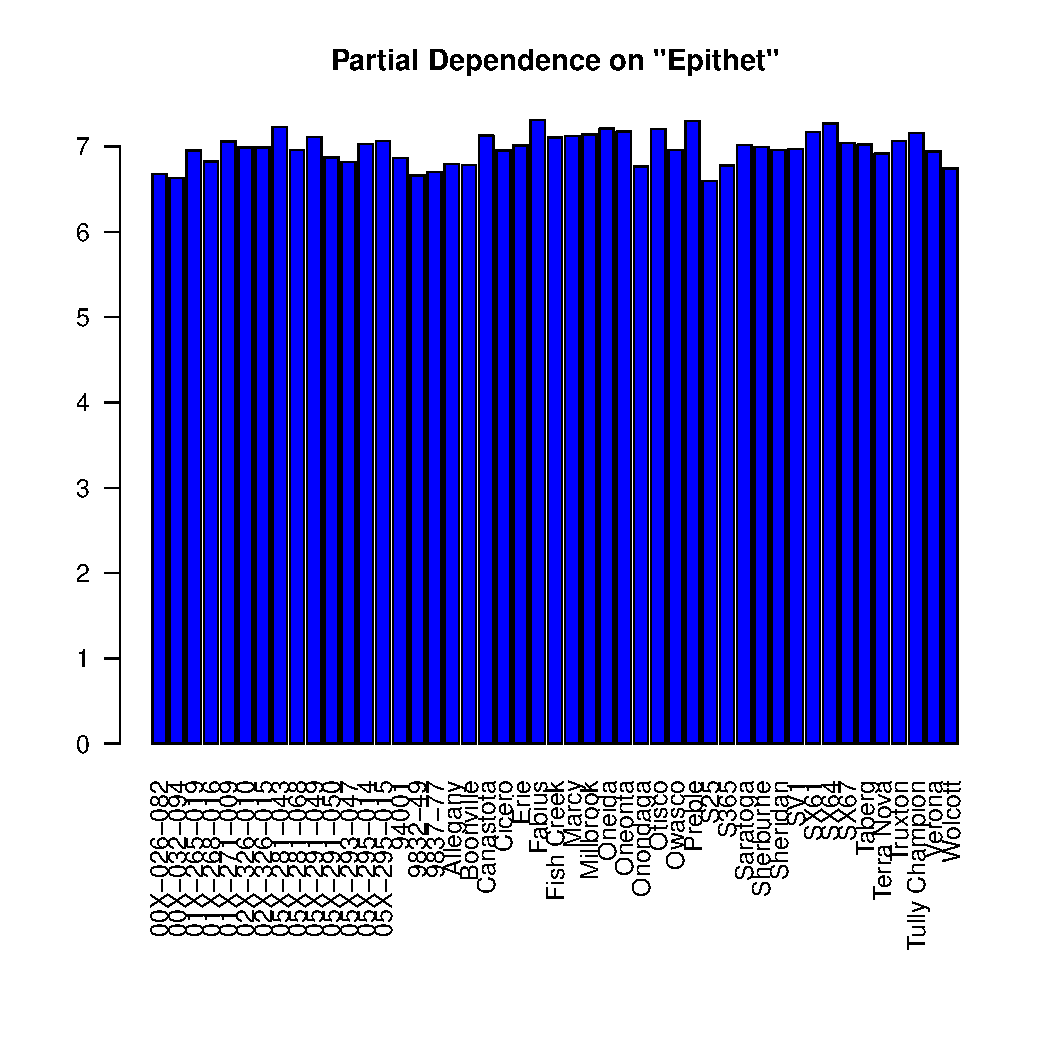
\includegraphics[width=\maxwidth]{figure/PartialDependence-5} 

}




{\centering 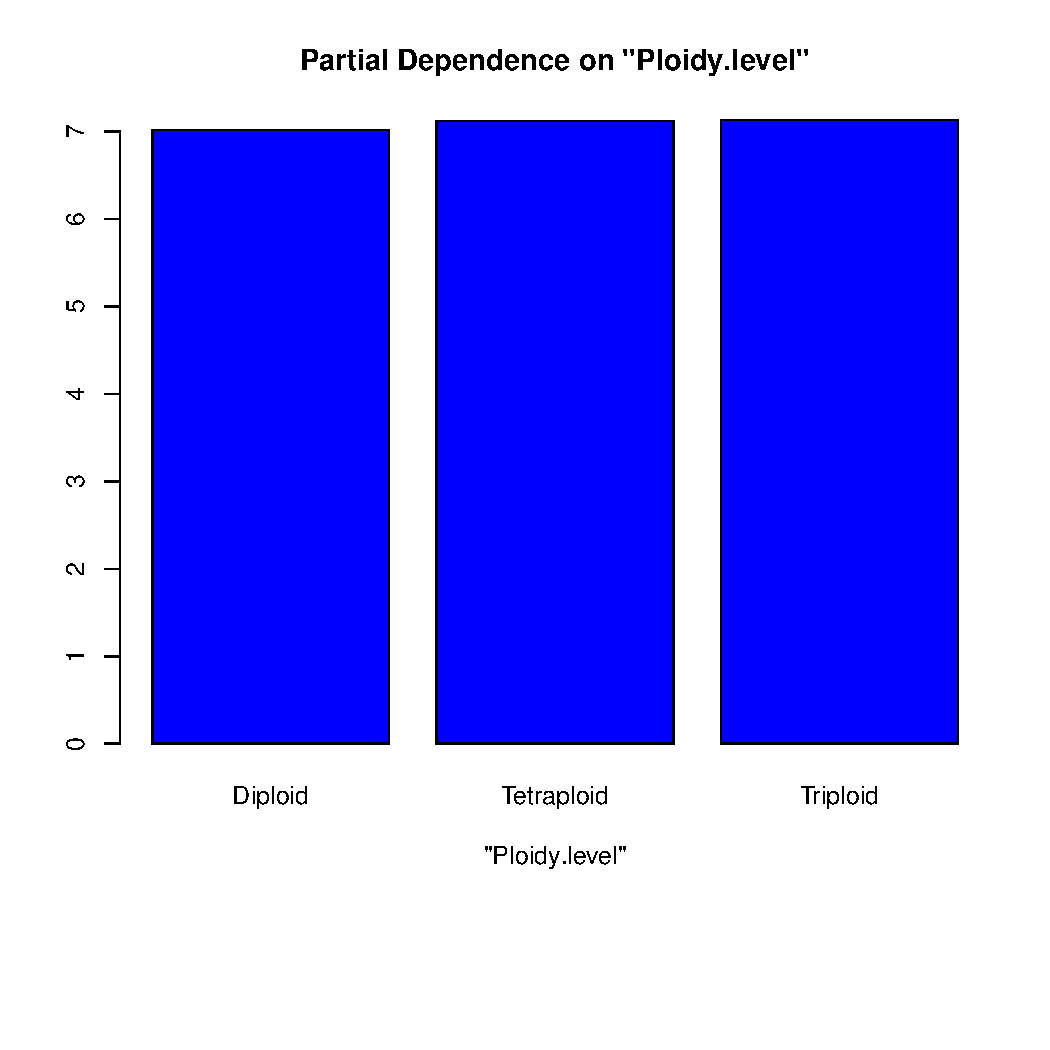
\includegraphics[width=\maxwidth]{figure/PartialDependence-6} 

}



\end{knitrout}
\\

The relationship between Survival (\%) and yield is not surprising but intriguing; having more than 80\% survival seems to be very important in predicting yield. This relationship has to be framed in the method used to measure survival; was it measured in the center 10 plants of the plot and not only on 4 plants where height was measured?  Also, how was yield calculated? the number of plants was included in the calculation? These questions would determine how valid is the relationship between survival and yield in the current experimental setup.\\

There is an interesting relationship between cellulose, lignin, ash content and yield. It seems that high yield is related with high concentration of cellulose and low concentration of lignin and ash. Therefore a variable that might be good exploring would be the ratio of concentration of cellulose/lignin or cellulose/(lignin + ash). I think the relationship between cellulose, lignin and ash is an indication of th epotential of the clone to grow biomass as well as the conditions in wich it grows. Based on Michelle's work on composition (you know more abouot it that I do) stressors like wind, or drought, high temperatures etc, would reduce the potential of the clone to produce biomass, represented mostly by cellulose, while increasing the need to produce stressor responses, represented by increased ligning and ash composition. This would be enhanced in clones that have high capacity to produce biomass. This is just a though and we can explore it more later... Waht do you think? \\


\begin{knitrout}
\definecolor{shadecolor}{rgb}{0.969, 0.969, 0.969}\color{fgcolor}

{\centering 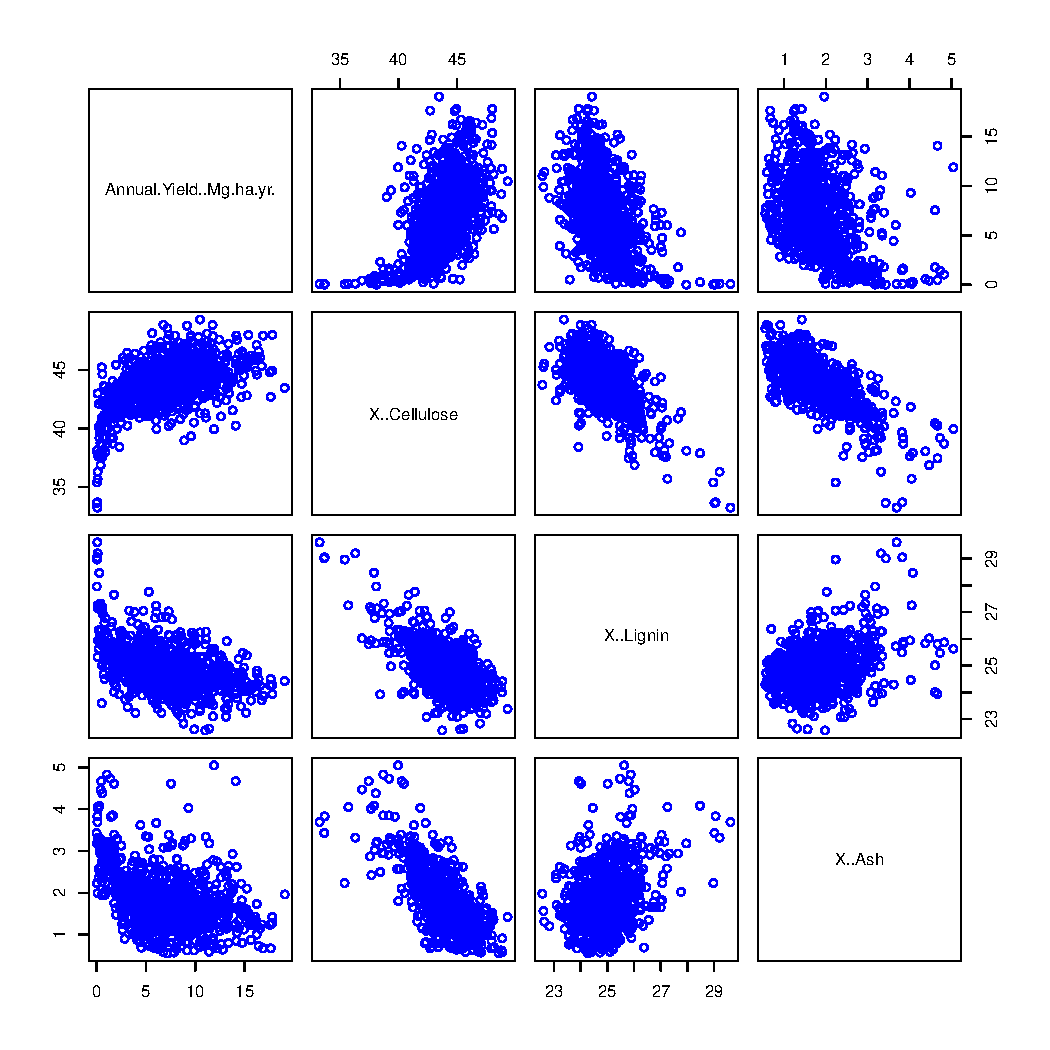
\includegraphics[width=\maxwidth]{figure/ScaterplotYieldComposition-1} 

}



\end{knitrout}
\\


Other interesting partial plots suggested by the variable importance results above are presented below.\\


\begin{knitrout}
\definecolor{shadecolor}{rgb}{0.969, 0.969, 0.969}\color{fgcolor}

{\centering 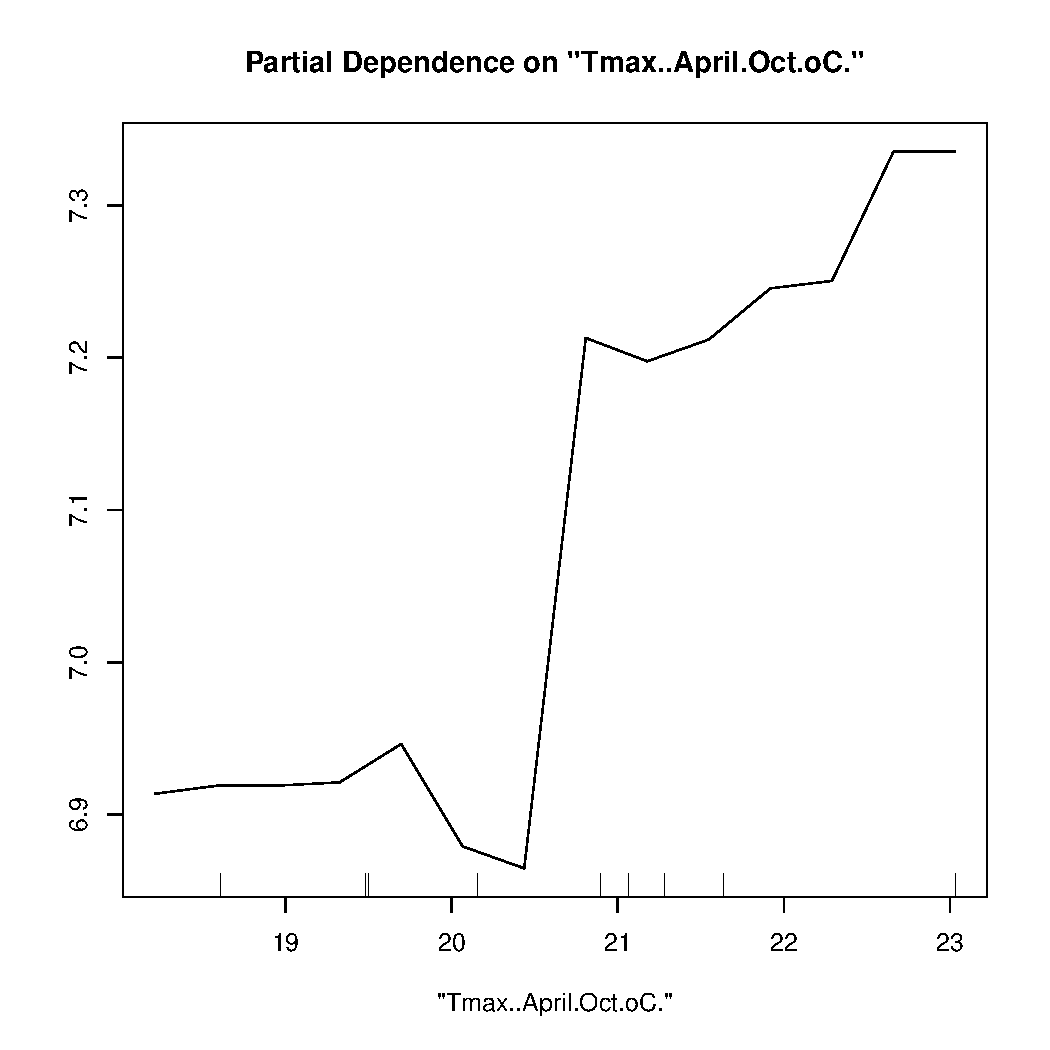
\includegraphics[width=\maxwidth]{figure/OtherPartialDependence-1} 

}




{\centering 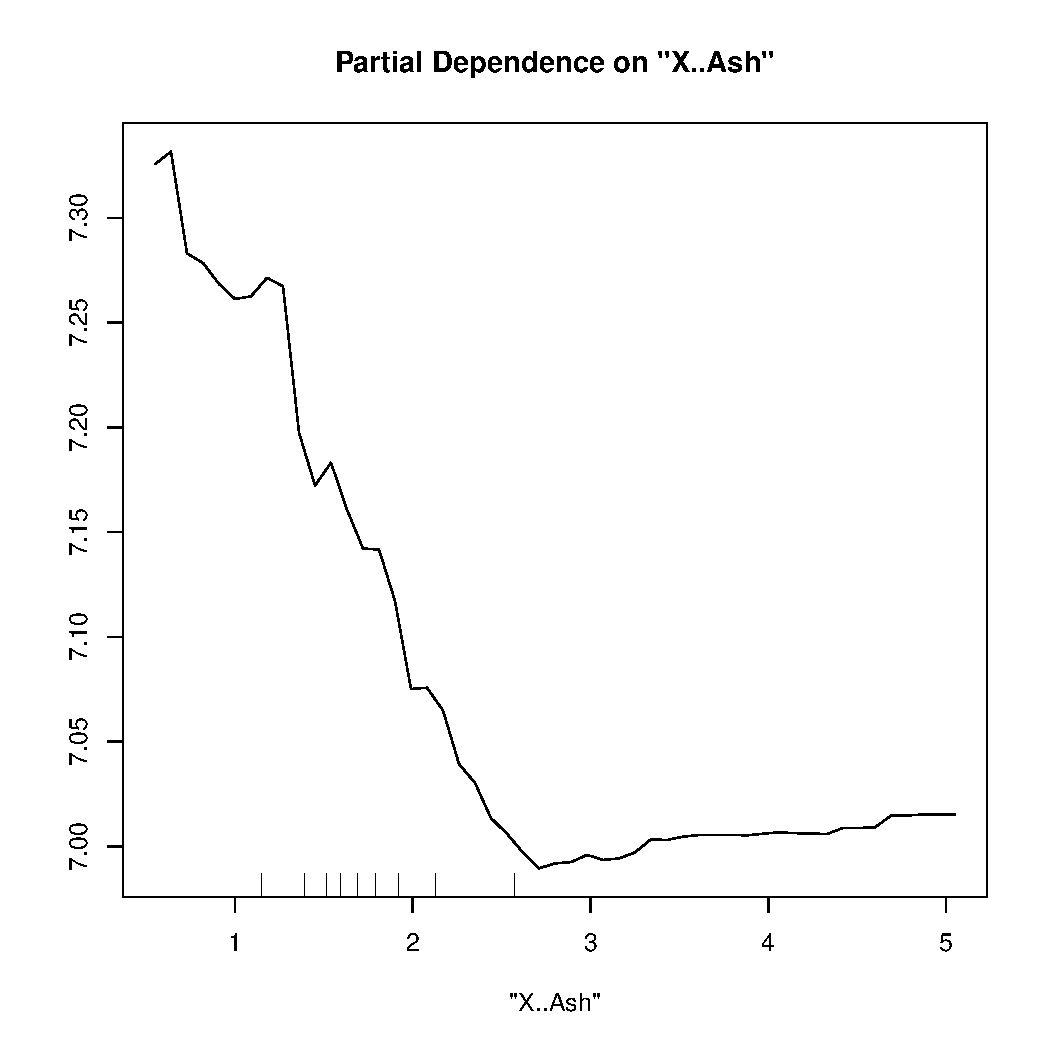
\includegraphics[width=\maxwidth]{figure/OtherPartialDependence-2} 

}




{\centering 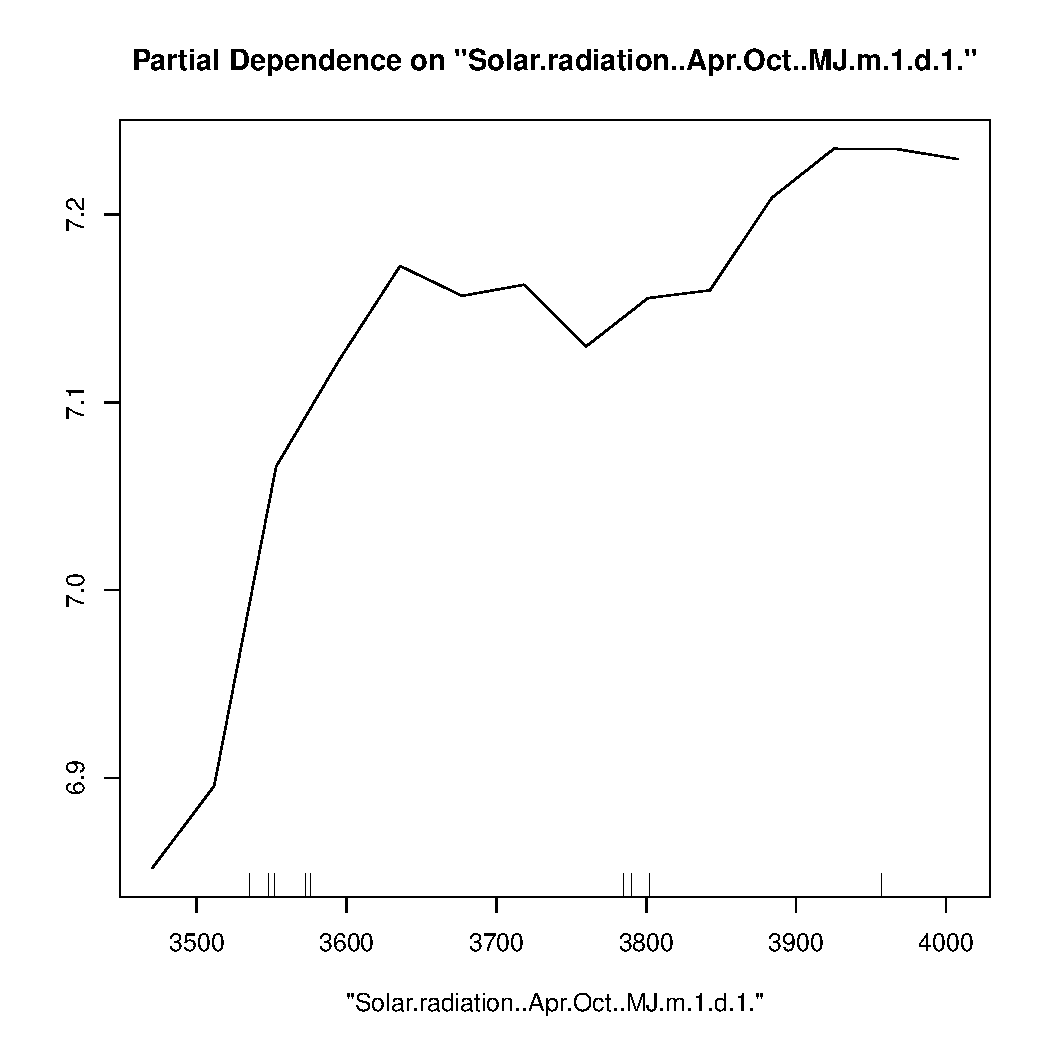
\includegraphics[width=\maxwidth]{figure/OtherPartialDependence-3} 

}




{\centering 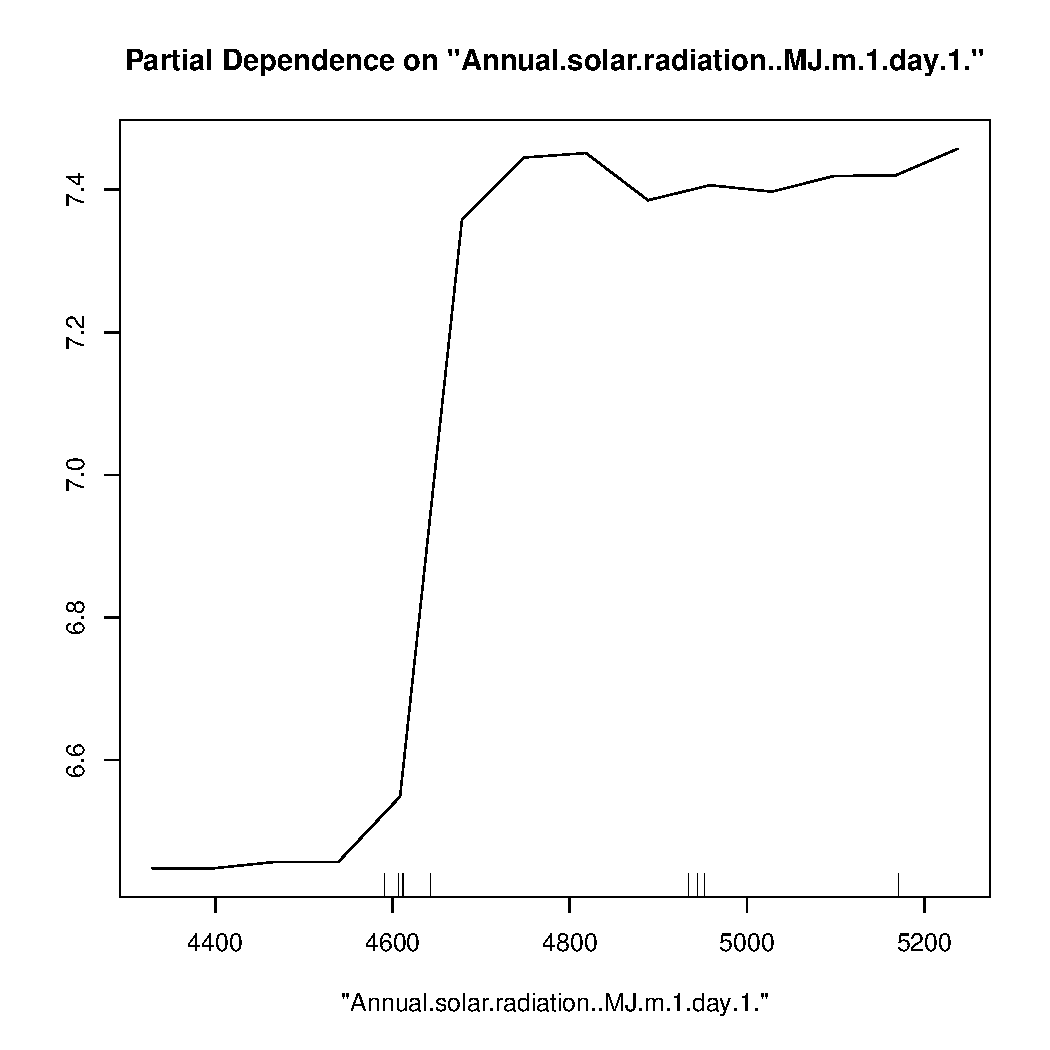
\includegraphics[width=\maxwidth]{figure/OtherPartialDependence-4} 

}




{\centering 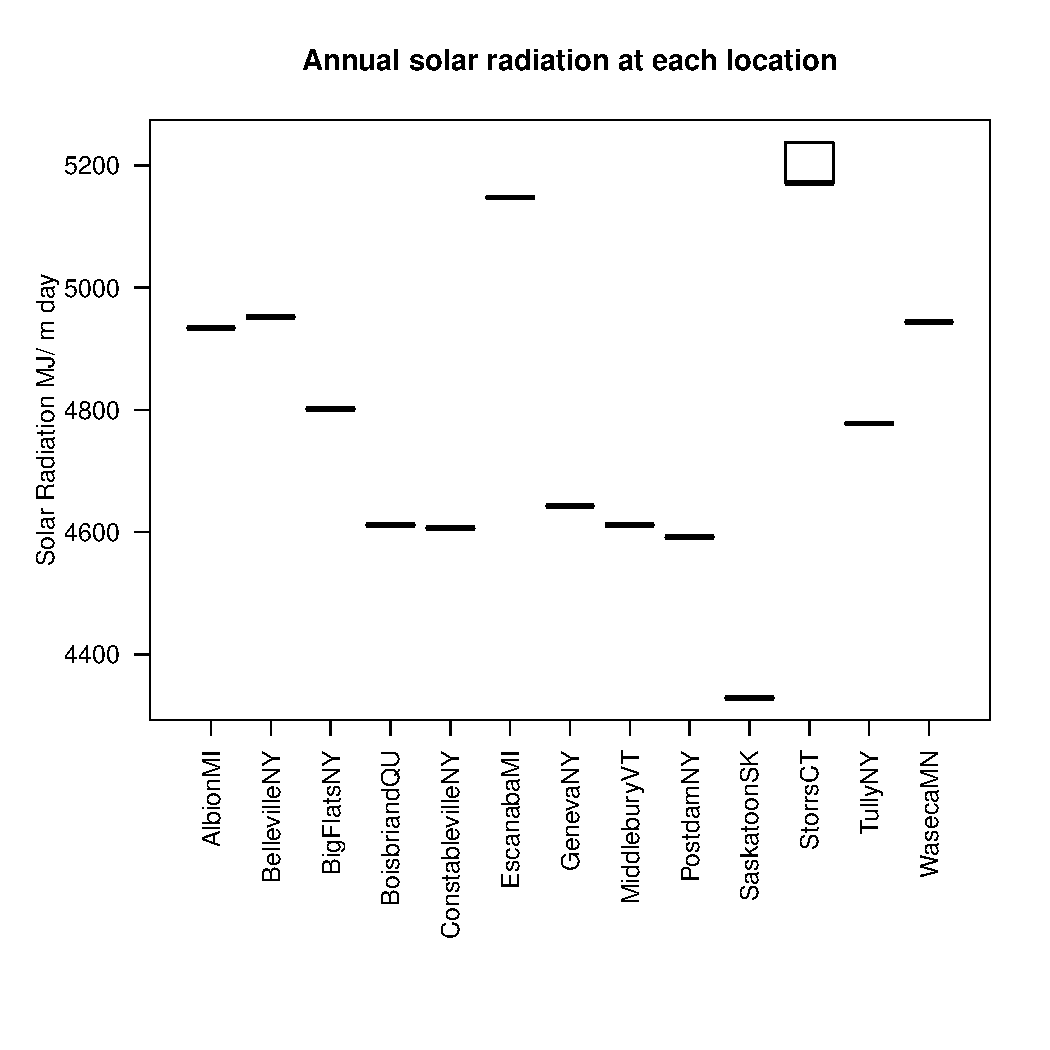
\includegraphics[width=\maxwidth]{figure/OtherPartialDependence-5} 

}



\end{knitrout}
\\

The interesting relationship between Annual solar radiation and Yield seen in the partial dependence plot, is explained by the plot of annual radiation at each location. Saskatoon, SK, has below 4400 MJ/ m day and is the only location at that level; the rest of the locations are between 4700 and 5200 MJ/ m day and there is not a particular significant trend in the relationship with yield and solar radiation in that range. 


\\

\begin{knitrout}
\definecolor{shadecolor}{rgb}{0.969, 0.969, 0.969}\color{fgcolor}

{\centering 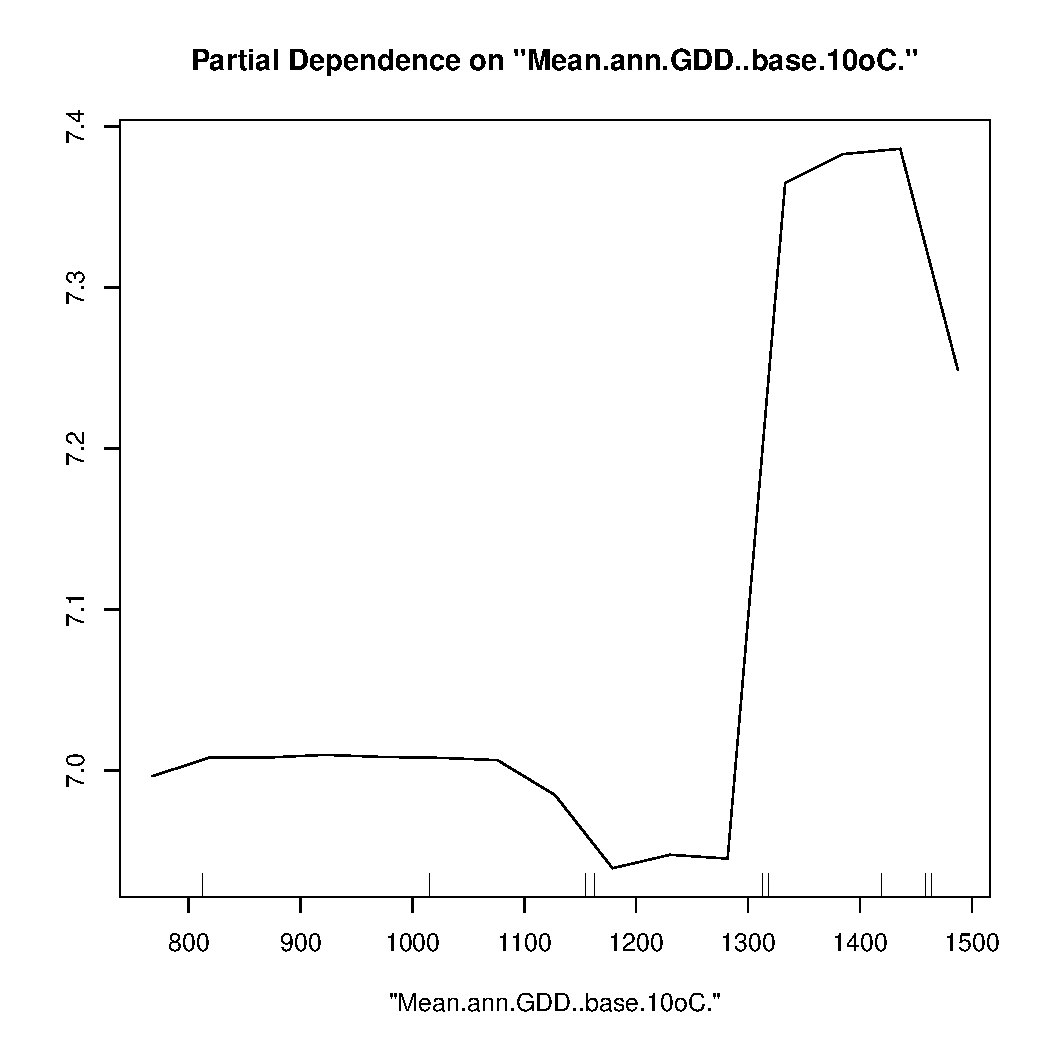
\includegraphics[width=\maxwidth]{figure/AdditionalPartialDependence-1} 

}




{\centering 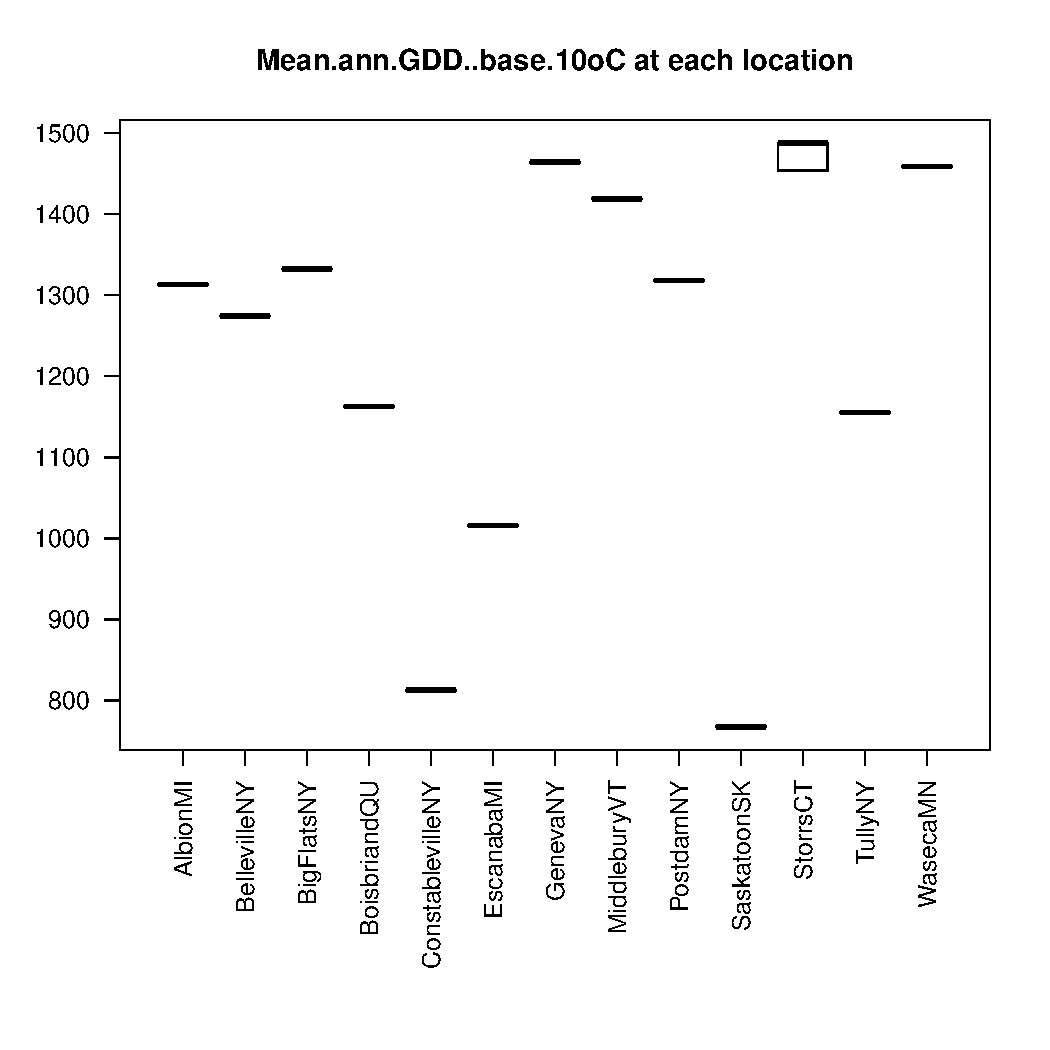
\includegraphics[width=\maxwidth]{figure/AdditionalPartialDependence-2} 

}



\end{knitrout}

\\

Similar to solar radiation, the partial dependence plot of yield and Mean GDD base 10 has an important change when GDD are between 1300 and 1450. Plotting the GDD for each location seems to indicate that locations between 1300 and 1450 have higher yields. That could be verified by computing the mean yileds for all the experiments in those locations. It something to consider for further analayis and for the genotype by environment relationship.


\subsubsection*{Proximity analysis }

The random forest algorithm creates a proximity measure between the variables base on how frequent they fall in the same final cathegory of the random tress making the forest. The more two variables end up in the same botom branch of the trees, the more 'similar' they are. It is equivalent to theprincipal component analysis in the AMMI analysis. Using multy dimensional scaling plots of the similarity matrix, clusters and other relationships can be inferred and further explored.Note that the axis of the plots are representing teh combination teh variable combination that maximize the variance in the data and therefore do not have direct meaning.
In the particular case of Yield the proximity matrix seems to indicate that four distinctive groups

\begin{knitrout}
\definecolor{shadecolor}{rgb}{0.969, 0.969, 0.969}\color{fgcolor}

{\centering 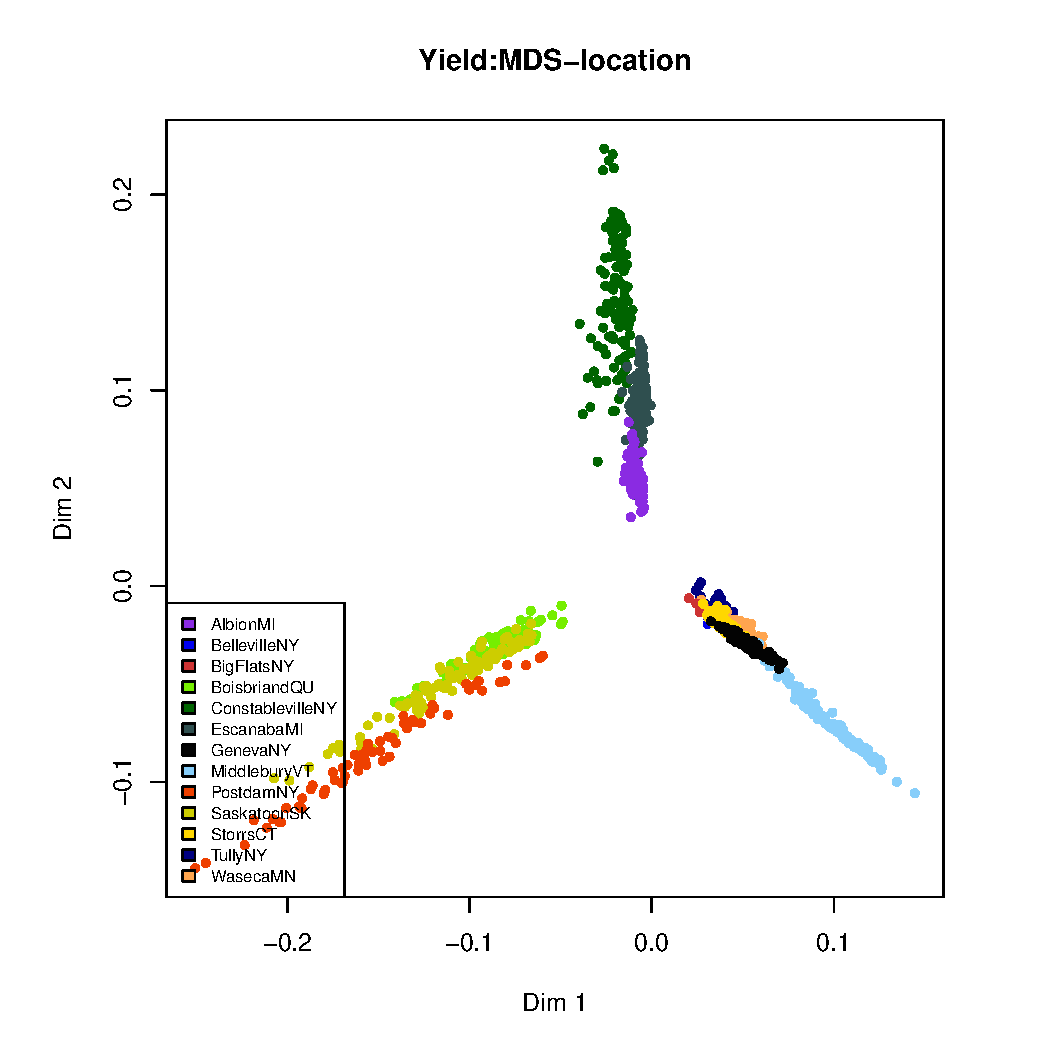
\includegraphics[width=\maxwidth]{figure/MSDSPlotsYield-1} 

}




{\centering \includegraphics[width=\maxwidth]{figure/MSDSPlotsYield-2} 

}




{\centering \includegraphics[width=\maxwidth]{figure/MSDSPlotsYield-3} 

}



\end{knitrout}

\\

The MDS proximity plots seem to indicate that the four groups are more related to location than to a genetic variables. Ploting the MSD proximity matrix with emphazising clone or ploidy does not indicate that genetic variables are important in the formation of the clusters.


% \subsection*{Random Forest analysis with clone as a response variable}
% 
% The random forest analaysis that we have performed so far can be fliped on its head and used to classify the genetic material, i.e. Clone ID, on the basis of all  the other variables. There is a more elaborate procedure that uses random forest analysis in the unsupervised mode to find patterns on the data, but is it quite complex and we should decide if it is worth ir once we decide which variables are worth doing this kind of analysis and of which section of the database.
% 
% The factor Clone ID was chosen to indicate the genetic material for the random forest analysis. This is a subjective choice made by me (Felipe) and can be changed if a better one is suggested by others in the group. Before proceeding with the random forest analysis on Clones, the database needs to be processed eliminating enties that does not have a Clone ID, as well as imputing missing variable of other variables. This can be modified as the group decides further along the analytic process. Clones with few entries are excluded from the analsysis to bring the levels of factor Clone ID below 53, as was done before.
% 


% 
% <<RandomForestClone,echo=FALSE,fig.align='center'>>=
% 
% plot(RF.Yield);
% 
% 
% @




\end{document}
